\documentclass[ordinary]{BMSTU-IU8}

\captionsetup[figure]{
    width=1.0\linewidth,
    justification=justified,
    font=small,
    name=Рисунок,
    labelsep=endash,
    position=below,
}

\captionsetup[table]{
    name=Таблица,
    labelsep=endash, % Тире
    position=above,
    justification=justified,
    singlelinecheck=false,
    font=small,
}

\usepackage{amssymb}

\addbibresource{main.bib}

\student{Н. В. Железцов}
\theme{Курсовая работа \\ Факторизация целых чисел с использованием сублинейных
       ресурсов на сверхпроводниковом квантовом процессоре}
\discipline{Криптографические методы защиты информации}
\group{ИУ8-104}

\supervisor{А. Е. Жуков}

\begin{document}
    \maketitle
    \setcounter{page}{3}

    \structure{РЕФЕРАТ}

Алгоритм Шора серьёзно поставил под вопрос безопасность информации, основанную
на криптосистемах с открытым ключом. Однако для взлома широко используемой
схемы RSA-2048 требуются миллионы физических кубитов, что значительно превышает
текущие технические возможности. Здесь мы сообщаем об универсальном квантовом
алгоритме факторизации целых чисел, объединяющем классическую редукцию базиса
решетки с квантовым алгоритмом приближённой оптимизации (QAOA). Количество
требуемых кубитов равно $O(\log N / \log\log N)$, что сублинейно относительно
битовой длины целого числа $N$, делая этот алгоритм самым экономичным по числу
кубитов алгоритмом факторизации на сегодняшний день. Мы экспериментально
демонстрируем алгоритм, факторизуя целые числа размером до 48 бит с помощью 10
сверхпроводящих кубитов, что является наибольшим целым числом, факторизованным
на квантовом устройстве. Мы оцениваем, что квантовая схема с 372 физическими
кубитами и глубиной в тысячи операций необходима для того, чтобы бросить вызов
RSA-2048 при помощи нашего алгоритма. Наше исследование демонстрирует
значительные перспективы для ускорения применения текущих шумных квантовых
компьютеров и прокладывает путь к факторизации больших целых чисел, имеющих
реальное криптографическое значение.

    \tableofcontents
    \structure{ВВЕДЕНИЕ}

Квантовые вычисления вступили в эпоху шумных квантовых устройств промежуточного
масштаба (NISQ) \cite{cite_1, cite_2}. Важной задачей эпохи NISQ является
демонстрация того, что устройства NISQ могут превзойти классические компьютеры
при решении задач с практической значимостью, то есть достижение практического
квантового преимущества. Алгоритмы, требующие минимальных ресурсов и
использующие ограниченное число доступных кубитов и глубину схем для решения
задач, сложных для классических вычислений, имеют особую важность. Вариационные
квантовые алгоритмы, использующие гибридную схему вычислений
«классика+квантовые вычисления», обладают значительным потенциалом для
получения значимого квантового преимущества в эпоху NISQ \cite{cite_3, cite_4,
cite_2, cite_5, cite_6}. Одним из таких алгоритмов является квантовый алгоритм
приближённой оптимизации (QAOA) \cite{cite_5}, первоначально предложенный для
решения задач на собственные значения, который впоследствии широко применялся в
различных областях, таких как химическое моделирование \cite{cite_7, cite_8},
машинное обучение \cite{cite_9}, а также инженерные приложения \cite{cite_10,
cite_11}.

Факторизация целых чисел является одной из важнейших основ современной
информационной безопасности \cite{cite_12}. Экспоненциальное ускорение
факторизации алгоритмом Шора \cite{cite_13} является выдающимся примером
превосходства квантовых вычислений. Однако выполнение алгоритма Шора на
отказоустойчивом квантовом компьютере требует значительных ресурсов
\cite{cite_14, cite_15}. На сегодняшний день наибольшее целое число,
факторизованное алгоритмом Шора на существующих квантовых системах, это число
21 \cite{cite_16, cite_17, cite_18}. Альтернативно, факторизация целых чисел
может быть сведена к задаче оптимизации, решаемой посредством адиабатических
квантовых вычислений (AQC) \cite{cite_19, cite_20, cite_21, cite_22} или QAOA
\cite{cite_23}. Более крупные числа были факторизованы этими методами на
различных физических системах \cite{cite_24, cite_25, cite_26, cite_27}.
Максимальные числа, факторизованные на данный момент, включают 291311 (19 бит)
в системе NMR \cite{cite_26}, 249919 (18 бит) на квантовом отжигателе D-Wave
\cite{cite_25}, 1099551473989 (41 бит) на сверхпроводящем устройстве
\cite{cite_27}. Однако следует отметить, что некоторые из факторизованных чисел
были специально подобраны с особыми структурами \cite{cite_28}, поэтому
наибольшее число, факторизованное универсальным методом на реальной физической
системе, на сегодняшний день составляет 249919 (18 бит).

В данной работе мы предлагаем универсальный квантовый алгоритм факторизации
целых чисел, требующий лишь сублинейные квантовые ресурсы. Алгоритм основан на
классическом алгоритме Шнорра \cite{cite_29, cite_30}, использующем редукцию
базиса решётки для факторизации целых чисел. Мы используем QAOA для оптимизации
наиболее трудоёмкой части алгоритма Шнорра, что ускоряет общее время
факторизации. Для целого числа $N$, имеющего $m$ бит, количество требуемых
кубитов в нашем алгоритме составляет $O(m / \log m)$, что сублинейно
относительно битовой длины числа $N$. Это делает наш алгоритм наиболее
экономным по числу кубитов по сравнению с существующими алгоритмами, включая
алгоритм Шора. С использованием данного алгоритма нами успешно факторизованы
числа 1961 (11 бит), 48567227 (26 бит) и 261980999226229 (48 бит) с
использованием, соответственно, 3, 5 и 10 кубитов на сверхпроводящем квантовом
процессоре. Число в 48 бит (261980999226229) также является наибольшим целым
числом, факторизованным универсальным методом на реальном квантовом устройстве.
Далее мы оцениваем квантовые ресурсы, необходимые для факторизации RSA-2048.
Согласно нашим расчётам, квантовая схема с 372 физическими кубитами и глубиной
порядка тысяч операций необходима для факторизации RSA-2048 даже в самой
простой одномерной системе. Подобный масштаб квантовых ресурсов, вероятно,
станет достижимым на устройствах NISQ в ближайшем будущем.



    \structure{ОСНОВНАЯ~ЧАСТЬ}

\section{Структура алгоритма}

\begin{figure}
    \centering
    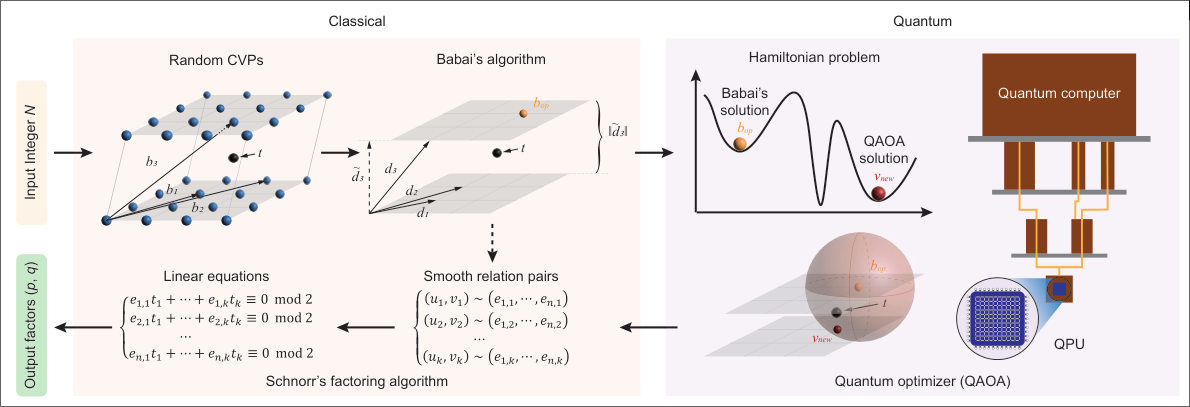
\includegraphics[scale=0.4]{inc/fig_01.png}
    \caption{
        Порядок работы квантового алгоритма факторизации целых чисел с
        сублинейными ресурсами (SQIF). Алгоритм использует гибридную
        «классическую+квантовую» структуру, в которой квантовый оптимизатор
        QAOA применяется для оптимизации классического алгоритма факторизации
        Шнорра. Сначала задача предварительно обрабатывается как задача
        ближайшего вектора (CVP) на решётке. Затем квантовый компьютер
        работает в качестве оптимизатора, уточняя классические векторы,
        полученные алгоритмом Бабая; на этом этапе находится решение CVP
        более высокого качества (то есть более близкое). Оптимизированные
        результаты передаются обратно в процедуру алгоритма Шнорра. После
        пост‑обработки в конце выводятся множители $p$ и $q$
    }
    \label{fig:fig01}
\end{figure}

Порядок работы квантового алгоритма факторизации целых чисел с сублинейными
ресурсами (SQIF) представлен на рис. \ref{fig:fig01}, который, по существу,
представляет собой гибридную «классическую+квантовую» структуру. Основная идея
состоит в использовании квантового оптимизатора QAOA для оптимизации самой
ресурсоёмкой части алгоритма Шнорра, что, в результате, повышает общую
эффективность процесса факторизации. Как показано на левой панели рис.
\ref{fig:fig01}, алгоритм Шнорра включает два существенных шага: поиск
достаточного количества пар гладких отношений (для краткости, sr‑пары) и
решение полученной системы линейных уравнений. Как правило, поиск sr‑пар
является самой важной и трудоёмкой частью алгоритма, тогда как решение системы
уравнений может быть выполнено за полиномиальное время. В алгоритме Шнорра
\cite{cite_31} задача sr‑пар преобразуется в задачу ближайшего вектора (CVP) на
решётке и решается посредством алгоритмов редукции базиса решётки, таких как
алгоритм Бабая \cite{cite_32}. Поскольку CVP является известной NP‑трудной
задачей \cite{cite_33}, мы можем рассчитывать только на приближённое, а не
точное решение CVP за полиномиальное или другое приемлемое время. Вероятность
получения sr‑пары пропорциональна качеству решения CVP \cite{cite_29}. То есть
чем ближе вектор‑решение CVP, тем эффективнее поиск sr‑пар. Исходя из
изложенного, мы предлагаем схему, в которой QAOA дополнительно оптимизирует
решение CVP, полученное алгоритмом Бабая. Полный процесс алгоритма SQIF
представлен в подробных примерах в \cite{cite_31}. В дальнейшем мы
сосредоточимся на квантовых этапах алгоритма.

Мы объединяем алгоритм Бабая с QAOA для решения CVP на решётке. Пусть дана
решётка $\Lambda$ с набором базиса $B=[b_1,\ldots,b_n]\in {R}^{(n+1)\times n}$
и целевой вектор ${t}\in{R}^{n+1}$. Алгоритм Бабая находит вектор
${b}_{{op}}\in\Lambda$, приближённо ближайший к ${t}$, в два шага. Сначала
выполняется LLL‑редукция с параметром~$\delta$ для заданного базиса~$B$. В
результате получаем LLL‑редуцированный базис $D=[d_1,\ldots,d_n]$ и
соответствующий ортогональный базис Грама–Шмидта
$\widetilde{D}=[\widetilde{d}_1,\ldots,\widetilde{d}_n]$. Второй шаг —
«уменьшение размера» целевого вектора ${t}$ с использованием
LLL‑редуцированного базиса. Так получаем приближённый ближайший вектор

\begin{equation}
    {b}_{{op}}
    = \bigl(b^{1}_{{op}},\ldots,b^{\,n+1}_{{op}}\bigr)^{\prime}
    = \sum_{i=1}^{n} c_{i}\,d_{i},
\end{equation}

где коэффициент $c_i=\lceil\mu_i\rfloor=
\left\lceil\langle{d},\widetilde{d}_i\rangle/
\langle\widetilde{d}_i,\widetilde{d}_i\rangle\right\rfloor$ получается
округлением к ближайшему целому коэффициента Грама–Шмидта~$\mu_i$. Здесь
следует отметить, что функция округления к ближайшему значению выполняет лишь
одно приближение за раз. Фактически, если значения двух функций округления
можно учесть одновременно, удаётся получить решение более высокого качества
\cite{cite_31}. Однако этот процесс экспоненциально увеличивает объём
классических операций, что неприемлемо для классического компьютера. Мы
применяем идею квантовых вычислений, используя суперпозицию кубитов для
одновременного кодирования значений коэффициентов, полученных двумя функциями
округления. Затем мы формулируем задачу оптимизации, основываясь на евклидовом
расстоянии между новым вектором решётки и целевым вектором. Подробности
построения приведены ниже.

Пусть $v_{new}$ — новый вектор, полученный случайным выбором $x_i\in\{0,\pm1\}$
на коэффициенте $c_i$, удовлетворяющий

\begin{equation}
    v_{new}
    \;=\;
    \sum_{i=1}^{n} (c_i + x_i)\,d_i
    \;=\;
    \sum_{i=1}^{n} x_i\,d_i + b_{op}.
\end{equation}

Мы определяем функцию потерь задачи оптимизации следующим образом

\begin{equation}
    F(x_{1},\ldots,x_{n})
    \;=\;
    \bigl\lVert t - v_{new} \bigr\rVert^{2}
    \;=\;
    \Bigl\lVert\,
        t - \sum_{i=1}^{n} x_i\,d_i - b_{op}
    \Bigr\rVert^{2}.
\end{equation}

Значение функции $\lVert t-v_{new}\rVert^{2}$ представляет собой квадрат
евклидова расстояния от нового вектора до целевого вектора. Чем меньше значение
функции потерь, тем ближе новый вектор к целевому вектору $t$ и тем выше
качество решения. Когда все переменные $x_{i,i=1,\ldots,n}$ принимают нулевые
значения, получаем оптимальное решение, выдаваемое алгоритмом Бабая.

Отображая переменную $x_i$ на операторы Паули‑$Z$, можно построить гамильтониан
задачи, соответствующий уравнению (3), в виде

\begin{equation}
    H_{C}
    \;=\;
    \Bigl\lVert
        t - \sum_{i=1}^{n} \hat{x}_{i}\,d_{i} - b_{op}
    \Bigr\rVert^{2}
    \;=\;
    \sum_{j=1}^{\,n+1}
    \Bigl|
    t_{j}
    - \sum_{i=1}^{n} \hat{x}_{i}\,d_{i,j}
    - b_{op}^{\,j}
    \Bigr|^{2}.
\end{equation}

где $\hat{x}_i$ — квантовый оператор, сопоставленный базису Паули‑$Z$ согласно
правилам однокубитного кодирования (см.~\cite{cite_31}).

В таком случае число кубитов, необходимых для квантовой процедуры оптимизации
алгоритма Бабая, равно размерности решётки. Согласно анализу из \cite{cite_31},
эта размерность удовлетворяет $n\sim 2c\log N/\log\log N$, где $c$ — параметр
решётки, близкий к 1. Следовательно, чтобы факторизовать $m$‑битное целое
число $N$, наш алгоритм требует $O(m/\log m)$ кубитов — сублинейную величину по
$m$, в то время как алгоритм Шора нуждается в $O(m)$ кубитах \cite{cite_13}, а
метод таблицы произведений — в $O(m^{2})$ кубитах \cite{cite_25}. Тем самым наш
алгоритм является самым экономичным по числу кубитов на сегодняшний день и
первым универсальным квантовым алгоритмом факторизации с сублинейными
квантовыми ресурсами.

    \section{Эксперимент и результаты}

Мы демонстрируем работу алгоритма, экспериментально факторизуя три целых числа
на сверхпроводящем квантовом процессоре, где выбраны десять кубитов и девять
соединителей, расположенных в топологии цепочки. Все кубиты и соединители — это
настраиваемые по частоте сверхпроводящие кубиты (transmon --- трансмон);
однокубитные вращения вокруг осей $x$ или $y$ сферы Блоха реализуются подачей
управляющих сигналов, в которых информация затвора закодирована в амплитуде и
фазе СВЧ‑импульсов. Виртуальные $z$‑затворы используются для выполнения
вращений вокруг оси $z$. Двухкубитные затворы с контролируемой файзой (CZ)
реализуются за счёт обмена совместными состояниями $|11\rangle$ и $|02\rangle$
(или $|20\rangle$) соседних кубитов, когда активируется взаимодействие,
передаваемое через соединитель \cite{cite_34}. Параллельные измерения
производительности кросс-энтропии (XEB --- cross-entropy benchmarking) дают
средние достоверности порядка $99{,}9\,\%$ для однокубитных вращений и
$99{,}5\,\%$ для CZ‑затворов. Подробности экспериментальной установки и
характеристики процессора приведены в \cite{cite_31}.

Мы факторизуем 11‑битное число $1961$, 26‑битное число $48567227$ и 48‑битное
число $261980999226229$, используя соответственно 3, 5 и 10 сверхпроводящих
кубитов. Ниже показан процесс получения одной sr‑пары квантовым методом в
каждой серии экспериментов. Вычисления остальных sr‑пар аналогичны и
выполняются численно; все sr‑пары и соответствующие системы линейных уравнений
приведены в \cite{cite_31}.

Топология $ZZ$‑слагаемых в гамильтониане задачи согласно уравнению (4)
представляет собой $K_n$ --- полный граф порядка $n$ \cite{cite_31}. Пример для
10 кубитов показан на рис. \ref{fig:fig02}B. Чтобы реализовать гамильтониан
типа $K_n$ на линейной 1D-цепочке физических кубитов, мы используем маршрутный
метод, основанный на классическом параллельном алгоритме пузырьковой
сортировки: все‑ко‑всем взаимодействия кубитов отображаются на взаимодействия
ближайших друг к другу двух кубитов с помощью cложных swap сетей, как показано
на рис. \ref{fig:fig02}D. Этот маршрутный метод является оптимальным и
добавляет лишь линейное увеличение глубины схемы. SWAP сети компилируются в
затворы рис. (рис. \ref{fig:fig02}E), которые могут исполняться непосредственно
на квантовом процессоре. Отметим маленький приём: чередование блоков ZZ‑SWAP
вверх‑вниз в чётных и нечётных слоях сетей позволяет сократить линейное число
затворов $H$.

\begin{figure}
    \centering
    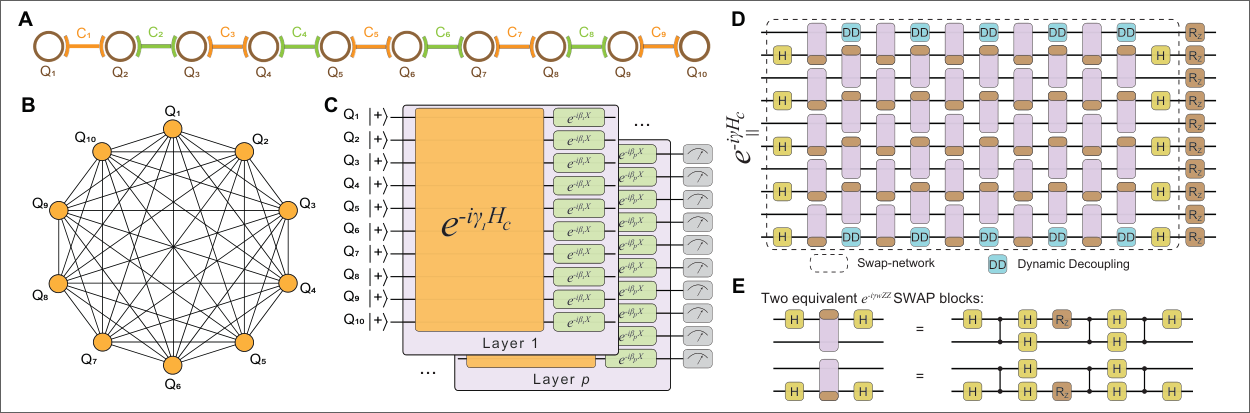
\includegraphics[scale=0.38]{inc/fig_02.png}
    \caption{
        Экспериментальная установка и схема QAOA алгоритма SQIF. \textbf{A}.
        Десять выбранных кубитов на сверхпроводящем квантовом процессоре;
        каждый кубит связан с ближайшими соседями через настраиваемые по
        частоте соединители. \textbf{B}. Родная топология взаимодействий
        гамильтониана задачи для случая факторизации на 10 кубитах,
        отображённая в линейную цепочку, показанную в A. \textbf{C}. Схема
        $p$‑слойного QAOA. Все кубиты инициализируются в состояние $|+\rangle$,
        далее следуют $p$ слоёв попеременного действия гамильтониана задачи
        (оранжевый) и смешивающего гамильтониана (зелёный) и завершающие
        измерения популяций (серый). Обратите внимание, что вариационные
        параметры $\{\gamma,\beta\}$ различны для каждого слоя. \textbf{D}.
        Маршрутная схема для отображения все‑к‑о‑всем гамильтониана 10 кубитов
        на линейную топологию ближайших соседей; построена «кирпичной» сеткой
        из двух одинаковых блоков SWAP с двумя слоями затворов $H$ (Hadamard) в
        начале и конце, за которыми следует слой затворов $R_z(\theta)$. Здесь
        угол вращения опущен. Глубина схемы пропорциональна числу
        задействованных кубитов. \textbf{E}. Подробная компиляция квантовой
        схемы в затворы сверхпроводящего квантового процессора.
    }
    \label{fig:fig02}
\end{figure}

QAOA находит приближённое основное состояние гамильтониана путём обновления
параметров (рис. \ref{fig:fig02}C; подробности см. \cite{cite_31}). Оптимизацию
параметров QAOA можно проиллюстрировать через ландшафт функции энергии
$E(\gamma,\beta)$. Сравнение теоретического и экспериментального ландшафтов
служит качественной диагностикой применимости QAOA на реальном оборудовании.
Для гиперпараметра $p=1$ ландшафт энергии как функция $(\gamma,\beta)$
изображён в 3D графике на рис. \ref{fig:fig03}. Значения энергии нормированы по
$E^{\ast}=(E-E_{\min})/(E_{\max}-E_{\min})$. На рис. \ref{fig:fig03} показаны
симуляция без шума (слева) и эксперимент (справа) для случаев 3, 5
и 10 кубитов. Различные цвета пикселей обозначают разные значения функции;
поверх наложена траектория сходимости классического оптимизатора (красная
кривая). Для оптимизации используется метод градиентного спуска по модели,
показавший хорошую работу как в теории, так и на практике. Алгоритм сходится в
область глобального минимума менее чем за 10 шагов во всех трёх случаях. Хотя
пути сходимости эксперимента отличаются от теоретических, они достигают
оптимума за сравнимое число шагов. Это свидетельствует об устойчивости
алгоритма к определённому уровню шума.

\begin{figure}
    \centering
    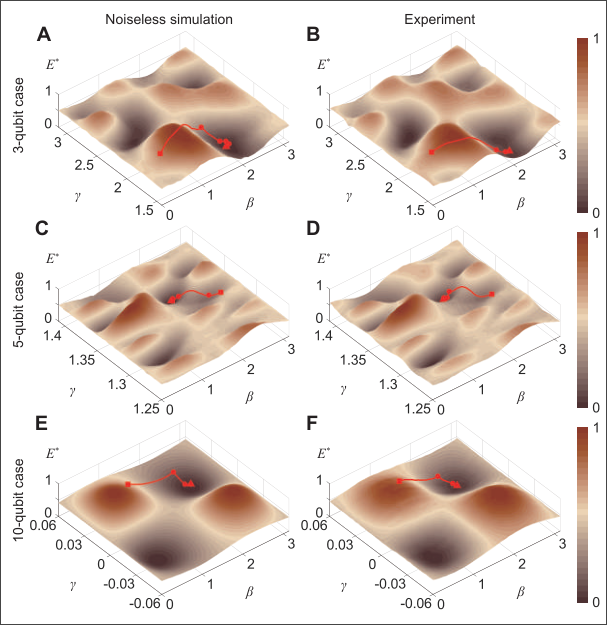
\includegraphics[scale=0.4]{inc/fig_03.png}
    \caption{
        Энергетические ландшафты и траектории сходимости QAOA при $p = 1$.
        \textbf{A}, \textbf{B} — численные и экспериментальные ландшафты для
        случая 3 кубитов; \textbf{C}, \textbf{D} — для 5 кубитов; \textbf{E},
        \textbf{F} — для 10 кубитов. В каждой экспериментальной группе оценены
        $41\times 41$ комбинаций $(\gamma,\beta)$, равномерно распределённых по
        сетке в подобласти всего двумерного пространства параметров. Для каждой
        точки сетки математическое ожидание энергии вычисляется по результатам
        $30\,000$ повторов схемы. Сравнение экспериментальных и численных
        ландшафтов демонстрирует отчётливое соответствие характерных
        особенностей. Наложенная траектория оптимизации (красная; стартует из
        квадратного маркера и сходится в треугольник) показывает способность
        классического оптимизатора находить оптимальные параметры.
    }
    \label{fig:fig03}
\end{figure}

В QAOA основная работа квантового компьютера состоит в подготовке квантовых
состояний с заданными вариационными параметрами. Теоретически
производительность QAOA улучшается с ростом глубины гиперпараметра $p$. Однако
с увеличением глубины накапливаются ошибки, и выгода может нивелироваться. Ниже
приведены результаты процессора при оптимальных $(\beta,\gamma)$. Мы
демонстрируем слои QAOA до $p=3$ для 3‑ и 5‑кубитных случаев и односоставную
QAOA ($p=1$) для 10 кубитов. Для 10 кубитов также выполнен запуск при $p=3$;
результат лучше случайного угадывания, но хуже, чем при $p=1$ \cite{cite_31}.
На рис. \ref{fig:fig04}A‑C видно, что вероятность целевого состояния (красная
пунктирная рамка) растёт с увеличением $p$. Хотя рост меньше теоретического, он
хорошо согласуется с шумовой симуляцией. Аналогичные результаты получены в
5‑кубитном эксперименте (рис. \ref{fig:fig04}D‑F). Для 10 кубитов при $p=1$
результаты показаны на рис. \ref{fig:fig04}G; для наглядности отображены 120
наиболее вероятных состояний по теории. Теоретическая вероятность целевого
состояния равна 0.02 (наибольшая), экспериментальная около 0.008, что близко к
шумовому значению 0.009. Экспериментальные результаты значительно превосходят
случайное угадывание 0.001, то есть вычислительный выигрыш QAOA остаётся
существенным. Более того, форма распределения вероятностей симметрична
относительно симуляционных данных, что также подтверждает хорошее совпадение
эксперимента с теорией.

\begin{figure}
    \centering
    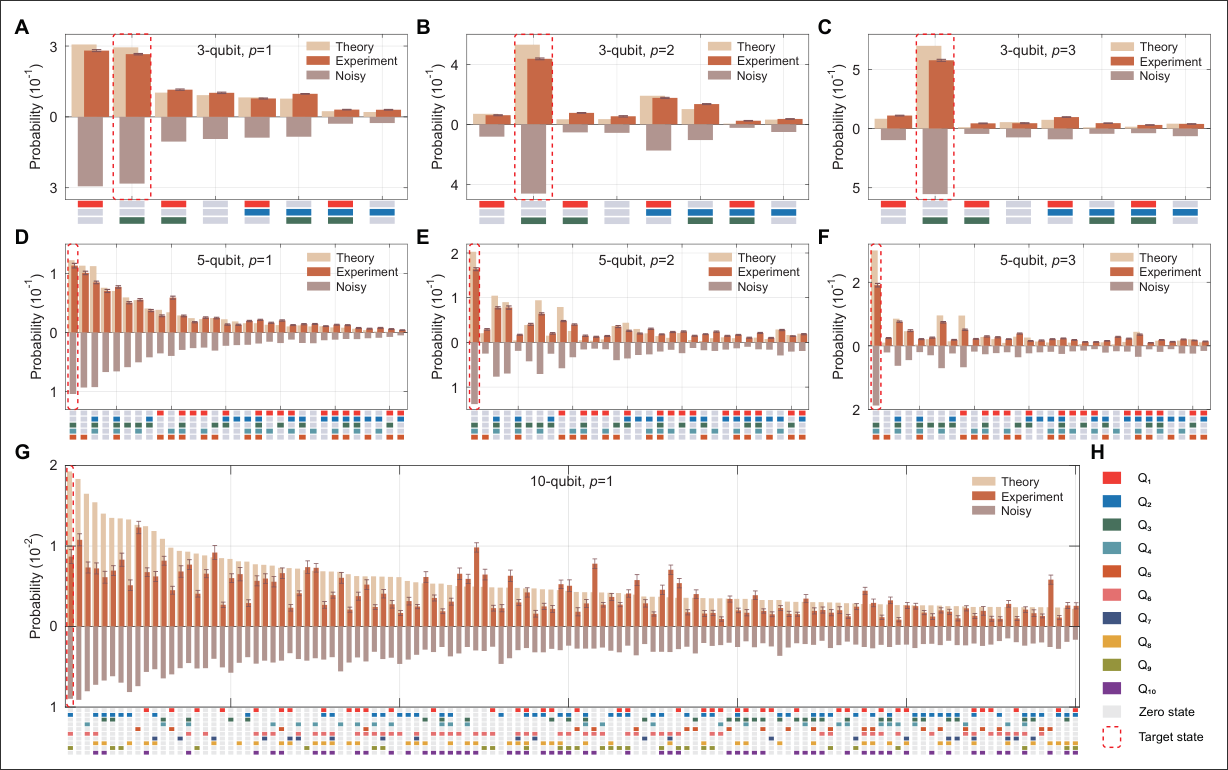
\includegraphics[scale=0.38]{inc/fig_04.png}
    \caption{
        Экспериментальная производительность QAOA для трёх случаев
        факторизации. \textbf{A–C}. Производительность QAOA для 3‑кубитного
        случая при $p = 1$, $p = 2$ и $p = 3$ соответственно. \textbf{D–F}.
        Производительность QAOA для 5‑кубитного случая при $p = 1$, $p = 2$
        и $p = 3$ соответственно. \textbf{G}. Производительность QAOA при $p =
        1$ для 10‑кубитного случая. Экспериментальные результаты, показанные
        оранжевым цветом, усреднены по 20 повторам эксперимента; штрихи ошибок
        отображают доверительный интервал в одном стандартном отклонении. Для
        сравнения также приведены теоретические (жёлтый) и шумовые при
        уровне 0.01 (серо‑тауповый) результаты. Видно, что все три группы
        экспериментальных данных на сверхпроводящем квантовом процессоре хорошо
        согласуются с теорией и шумовой моделью 0.01. \textbf{H}. Обозначения
        цветовых блоков, соответствующих базисным состояниям различных кубитов
        в подписи оси $x$.
    }
    \label{fig:fig04}
\end{figure}


    \section{Оценка квантовых ресурсов}

Ниже приведены квантовые ресурсы, необходимые для того чтобы поставить под
угрозу некоторые реальные числа RSA, основываясь на алгоритме SQIF, который
описан в данной работе. Основные упоминаемые ресурсы — число кубитов и глубина
квантовой схемы одного слоя QAOA. Как правило, квантовые схемы нельзя запускать
на квантовых устройствах напрямую, поскольку их проект не учитывает топологию
связей реальных физических систем. Исполнение часто требует дополнительных
ресурсов — вспомогательных кубитов и увеличения глубины схем. Мы рассмотрели
ресурсы для трёх типовых топологий: полностью связанной системы ($K_n$),
двумерной решётки (2DSL --- 2D-lattice system) и одномерной линейной цепочки
(LNN --- 1D-chain system). Мы показываем на конкретных схемах, что встраивание
не требует лишних кубитов, а глубина одного слоя QAOA остается $O(n)$ во всех
трёх случаях. Следовательно, для факторизации целых чисел нашим алгоритмом
необходимы сублинейные квантовые ресурсы. Возьмём RSA‑2048 в качестве примера,
в этом случае требуемое число кубитов $n = {2 \cdot 2048} / {\log 2048} \approx
372$. Глубина одного слоя QAOA составляет $1118$ для топологии $K_n$, $1139$
для 2DSL и $1490$ для самой простой LNN, что достижимо для устройств NISQ в
ближайшем будущем. Квантовые ресурсы для разных длин чисел RSA приведены в
таблице \ref{tab:tab1}. Подробный анализ дан в \cite{cite_31}.

\begin{table}[h]
    \centering
    \caption{
        Оценка ресурсов для чисел RSA. Основные квантовые ресурсы включают
        число кубитов и глубину квантовой схемы QAOA с одной итерацией в трёх
        типовых топологиях: полностью связанной системе ($K_n$), двумерной
        решётке (2DSL) и линейной цепочке (LNN). Результаты получены без учёта
        нативной компиляции базового модуля ZZ (или базового модуля ZZ‑SWAP) в
        конкретной физической системе.
    }
    \begin{tabular}{lrrrr}
        \hline\hline
        \text{RSA number} & \text{Qubits} & \text{$K_n$‑depth} &
        \text{2DSL‑depth} & \text{LNN‑depth} \\
        \hline
        RSA‑128  &  37 &  113 &  121 &  150 \\
        RSA‑256  &  64 &  194 &  204 &  258 \\
        RSA‑512  & 114 &  344 &  357 &  458 \\
        RSA‑1024 & 205 &  617 &  633 &  822 \\
        RSA‑2048 & 372 & 1118 & 1139 & 1490 \\
        \hline\hline
    \end{tabular}
    \label{tab:tab1}
\end{table}


    \conclusion

В ходе прохождения практики был проведён комплексный анализ механизма
шардирования в СУБД Tarantool. Основное внимание было уделено изучению
архитектуры модуля \texttt{vshard}, принципов распределения данных и
обеспечения согласованности при выполнении операций в шардированном кластере.

Были рассмотрены и проанализированы существующие подходы к реализации
Map-Reduce запросов по репликам. В результате исследования выявлены ключевые
проблемы, связанные с обеспечением консистентности данных при выполнении
распределённых запросов, и предложена альтернативная реализация.

Практическая значимость работы заключается в:
\begin{itemize}
    \item Систематизации знаний о работе шардированного кластера Tarantool;
    \item Выявлении ограничений существующей реализации модуля \texttt{vshard};
    \item Разработке предложений по расширению функциональности для поддержки
        Map-Reduce операций по репликам.
\end{itemize}

Полученные результаты могут быть использованы для дальнейшего развития модуля
шардирования Tarantool и улучшения его безопасности. Проведённое исследование
демонстрирует важность комплексного подхода к проектированию распределённых
систем и необходимость тщательного анализа требований к согласованности данных.

Результаты работы подтверждают возможность реализации эффективного механизма
выполнения Map-Reduce запросов по репликам в шардированной среде с соблюдением
требований к консистентности данных и производительности системы.

    \printbibliography

    \appendix
    \appendixsection{Основы теории решёток}

В последние годы решётки служат алгоритмическим инструментом для решения
широкого круга задач в информатике, математике и криптографии, особенно в
квантовоустойчивых криптографических протоколах. Ниже приведены базовые понятия
и известные алгоритмы, тесно связанные с нашей работой.

\subsection*{Базовые понятия}

Пусть $\lVert\cdot\rVert$ — евклидова норма векторов из $R^{m}$. Векторы
отмечаем полужирным (в переводе этого нет), матрицы пишем построчно; элементы
матрицы $M$ обозначаем $m_{i,j}$. Верхний индекс~$T$ — транспонирование.

\begin{itemize}
\item \textbf{Решётка.} Пусть $b_{1},\ldots,b_{n}\in R^{m}$ — линейно
        независимые столбцы, тогда множество всех линейных комбинаций их
        целочисленных коэффициентов — решётка, определяемая как
        \begin{equation} \Lambda(B) =\{\,Bx \mid x\in Z^{n}\,\} =\{\,b =
            x_{1}b_{1}+\dots+x_{n}b_{n} \mid x_{1},\dots,x_{n}\in Z\,\}.
        \end{equation} где $B=[b_{1},\ldots,b_{n}]\in R^{m\times n}$ — матрица
        базиса, которая также может быть использована чтобы представлять
        решетку для простоты. $\{b_1, \ldots, b_n\}$ - группа базиса решетки.
        Размерность решётки $n$. Её детерминант $\det\Lambda=(\det
        B^{T}B)^{1/2}$, здесь $B^T$ - транспонированная матрица $B$. При
        квадратной $B$ имеем $\det\Lambda=\det B$. Детерминант представляет
        объём решётки в геометрическом представлении, обозначается как
        $\operatorname{vol}(\Lambda)$. Длина точки $b\in R^{m}$ определяется
        как $\lVert b\rVert=(b^{T}b)^{1/2}$.

\item \textbf{Последовательные минимумы.} Для $n$‑мерной решётки $\Lambda$
        положительные числа $\lambda_{1}(\Lambda)\le\lambda_{2}(\Lambda)
        \le\dots\le\lambda_{n}(\Lambda)$ называются последовательными
        минимумами, где $\lambda_{k}(\Lambda)$ — наименьший радиус шара с
        центром в нуле, содержащего $k$ линейно независимых векторов из
        $\Lambda$. Обозначим $\lambda_{1}=\lambda_{1}(\Lambda)$ как длину
        кратчайшего ненулевого вектора из $\Lambda$.

\item \textbf{Постоянная Эрмита.} Эрмитовым инвариантом решётки $\Lambda$
        называется
        \begin{equation}
          \gamma(\Lambda)
          = \frac{\lambda_{1}^{2}(\Lambda)}{\operatorname{vol}(\Lambda)^{2/n}}
          = \frac{\lambda_{1}^{2}(\Lambda)}{\det(\Lambda)^{2/n}}.
        \end{equation}

        Постоянная Эрмита $\gamma_{n}$ — максимальное значение $\gamma(\Lambda)$
        для всех $n$‑мерных решёток, или минимальное константное $\gamma$,
        удовлетворяющее $\lambda_{1}(\Lambda)^{2}\le\gamma(\det\Lambda)^{2/n}$
        для всех решёток размености $n$ соответственно.

\item \textbf{QR‑разложение.} У решёточной матрицы базиса $B$ есть единственное
        разложение $B=QR\in R^{m\times n}$, где $Q\in R^{m\times n}$,
        $R=[r_{i,j}]_{1\le i,j\le n} \in R^{n\times n}$, здесь $Q\in R^{m\times
        n}$ — изомет­рическая (столбцы ортогональны и единичной длины), а $R
        \in R^{n\times n}$ — верхнетреугольная матрица с положительными
        диагональными элементами $r_{i,i}$. Коэффициенты Грама–Шмидта
        $\mu_{j,i}=r_{i,j}/r_{i,i}$ легко вычисляются из QR‑разложения. Для
        целочисленной $B$ коэффициенты $\mu_{j,i}$ обычно рациональны.

\item \textbf{Задача кратчайшего вектора (SVP).}
      Дана группа базиса $B$ решётки $\Lambda$.

      \begin{itemize}
          \item Задача кратчайшего вектора (SVP): Требуется найти вектор
              $v\in\Lambda$, такой что $\lVert v\rVert=\lambda_{1}(\Lambda)$.
          \item Приближённая задача кратчайшего вектора ($\alpha$‑SVP): Найти
              ненулевой вектор $v\in\Lambda$, удовлетворяющий
              $\lVert v\rVert\le\alpha\,\lambda_{1}(\Lambda)$.
          \item Эрмитова задача кратчайшего вектора ($r$‑Hermite SVP):
              Найти ненулевой вектор $v\in\Lambda$, такой что
              $\lVert v\rVert \;\le\; r\,\det(\Lambda)^{1/n}$.
      \end{itemize}

      Параметр $\alpha\ge1$ в $\alpha$‑SVP называется фактором аппроксимации.
      Обычнро задача упрощается при увеличении $\alpha$. При $\alpha=1$ задачи
      $\alpha$‑SVP и SVP совпадают. Истинное значение $\lambda_{1}$ в
      $\alpha$‑SVP трудно вычислить из-за сложности SVP, поэтому решение
      $\alpha$‑SVP не всегда легко проверить. Задача $r$‑Hermite SVP является
      вычислимой (относительно просто вычислимой), она определяется величиной
      $\det(\Lambda)^{1/n}$ вместо $\Lambda_1$. В результате, мы можем лешко
      проверить решение, но не можем сравнить его с кратчайшим вектором.

\item \textbf{Задача ближайшего вектора (CVP)}
      Дана группа базиса $B$ решётки $\Lambda$ и целевой вектор
      $t\in\operatorname{span}(B)$.

      \begin{itemize}
          \item Задача ближайшего вектора (CVP): Найти вектор $v\in\Lambda$,
              такой что расстояние $\lVert v - t\rVert$ может быть минимизировано,
              т.е. $\lVert v - t\rVert = \operatorname{dist}(\Lambda,t)$.
          \item $\alpha$-приближенная задача ближайшего вектора ($\alpha$‑CVP):
              Найти вектор $v\in\Lambda$, такой что расстояние
              $\lVert v - t\rVert \le \alpha \times \operatorname{dist}(\Lambda,t)$
          \item $r$-приближенная задача ближайшего вектора (($r$‑AbsCVP):  Найти
              $v\in\Lambda$ такое, что $\lVert v - t\rVert \le r$.
      \end{itemize}

      Определения аналогичны случаям для SVP; параметр $\alpha\ge1$ в
      $\alpha$‑CVP играет ту же роль, что и в $\alpha$‑SVP. В $r$‑AbsCVP
      параметр $r$ может быть любым разумным значением, соизмеримым с
      $\operatorname{dist}(\Lambda,t)$, например $\det(\Lambda)^{1/n}$ в
      $r$‑Hermite SVP.
\end{itemize}

\subsection*{Алгоритм LLL}
\begin{algorithm}[htp!]
    \SetAlgoLined

    \KwData{базис решётки $\text{b}_1, \dots, \text{b}_n \in \text{Z}^m$, параметр $\delta$}
    \KwResult{$\delta$-LLL-редуцированный базис}

    \textbf{Шаг 1:} Орторгонализация Грама-Шмидта \\
    Выполнить орторгонализацию Грама-Шмидта для базиса $\text{b}_1, \dots, \text{b}_n$, обозначим результат как $\tilde{\text{b}}_1, \dots, \tilde{\text{b}}_n \in \text{R}^m$

    \textbf{Шаг 2:} Редукция

    \For{$i = 2$; $i < n$; $i = i + 1$}{
        \For{$j = i-1$; $i > 1$; $ i = i - 1$}{
            $c_{i,j} = \left\lfloor \dfrac{\langle \text{b}_i, \tilde{\text{b}}_j \rangle}{\langle \tilde{\text{b}}_j, \tilde{\text{b}}_j \rangle} \right\rceil$; \\
            $\text{b}_i \gets \text{b}_i - c_{i,j} \cdot \text{b}_j$;
        }
    }

    \textbf{Шаг 3:} Обмен

    \If{$\exists \, i$ такое, что $\delta \cdot \| \tilde{\text{b}}_i \|^2 > \| \mu_{i+1,i} \tilde{\text{b}}_i + \tilde{\text{b}}_{i+1} \|^2$}{
        $\text{b}_i \leftrightarrow \text{b}_{i+1}$; \\
        перейти к шагу 1;
    }

    \textbf{Шаг 4:} Вывод базиса $\text{b}_1, \dots, \text{b}_n$

    \caption{Алгоритм LLL-редукции}
    \label{alg:lll}
\end{algorithm}

Алгоритм LLL — один из самых известных алгоритмов редукции решётки; он был
предложен А. К. Ленстрой, Х. В. Ленстрой (мл.) и Л. Ловашем в 1982 г.
\cite{cite_35}. Для $n$‑мерной решётки этот алгоритм позволяет решать $\alpha
\;=\; \left(\frac{2}{\sqrt{3}}\right)^{n}$ за полиномиальное время. Ниже
приведены связанные понятия и алгоритмы.

\newcounter{tmp-enum-lll}

\begin{itemize}
    \item \textbf{LLL базиc}: Базис $B = QR$ называется LLL‑редукции или
        LLL‑базисом при параметре редукции $\delta\in(1/4,1]$, если выполняются
        условия:
        \begin{enumerate}
            \item $\frac{\lvert r_{i,j}\rvert}{r_{i,i}} \;\le\; \frac12, \quad \text{for all } j > i;$
            \item $\delta\, r_{i,i}^{2}\;\le\;r_{i,i+1}^{2} + r_{i+1,i+1}^{2},\quad \text{for } i = 1,\ldots,n-1.$
            \setcounter{tmp-enum-lll}{\value{enumi}}
        \end{enumerate}

        Очевидно, LLL‑базис также удовлетворяет
        \( r_{i,i}^{2} \le \alpha\, r_{i+1,i+1}^{2} \),
        для \(\alpha = \frac{1}{(\delta - 1 / 4)}\).

        Параметры, рассматриваемые в оригинальной литературе по алгоритму LLL,
        равны $\delta = \tfrac34$, $\alpha = 2$. Известный результат о LLL‑базисе
        показывает, что для любого $\delta < 1$ LLL‑базис может быть получен за
        полиномиальное время и хорошо аппроксимирует последовательные минимумы\:

        \begin{enumerate}
            \setcounter{enumi}{\value{tmp-enum-lll}}
            \item $\alpha^{-\,i+1} \;\le\; \lVert b_{i}\rVert^{2}\,\lambda_{i}^{-2}
                \;\le\; \alpha^{\,n-1}, \quad \text{for } i = 1,\ldots,n;$
            \item $\lVert b_{1}\rVert^{2} \;\le\; \alpha^{\frac{n-1}{2}}\,
                \bigl(\det\Lambda\bigr)^{2/n}.$
        \end{enumerate}

    \item \textbf{Алгоритм LLL}: Для заданного набора базиса
        $B = [b_{1},\ldots,b_{n}] \in Z^{m\times n}$
        алгоритм может привести его к LLL‑редуцированному виду
        или преобразовать в LLL‑базис. Алгоритм состоит из трёх
        основных шагов: ортогонализация Грама–Шмидта, редукции и
        обмен. Конкретные шаги приведены в Алгоритме \ref{alg:lll}.
\end{itemize}

\subsection*{Алгоритм ближайшей плоскости Бабая}

Алгоритм ближайшей плоскости Бабая \cite{cite_32} (далее — алгоритм Бабая)
применяется для решения CVP. Для $n$‑мерной решётки он может получать фактор
аппроксимации $\alpha \;=\; 2\!\left(\frac{2}{\sqrt{3}}\right)^{n}$ для
$\alpha$‑CVP. Алгоритм состоит из двух этапов, первый из которых заключается в
редукции решетки с помощью алгоритма LLL. Второй является процедурой уменьшения
размера, который в основном вычисляет линейную комбинацию целочисленных
коэффициентов, ближайших к целевому вектору $t$ в LLL-базисе. Этот шаг по сути
совпадает со вторым шагом в LLL-редукции. Подробные действия приведены в
Алгоритме \ref{alg:babai}.

\begin{algorithm}[htp!]
    \SetAlgoLined

    \KwData{базис решётки $\text{b}_1, \dots, \text{b}_n \in \text{Z}^m$, параметр $\delta = 3/4$, целевой вектор $\text{t} \in \text{Z}^m$}
    \KwResult{вектор $\text{x} \in \Lambda(B)$, такой что $\|\text{x} - \text{t}\| \leq 2^{n/2} \, \text{dist}(\text{t}, \Lambda(B))$}

    \textbf{Шаг 1:} LLL-редукция \\
    Применить LLL-редукцию к базису $B$ с параметром $\delta$ \\
    Обозначим результат: $\tilde{\text{b}}_1, \dots, \tilde{\text{b}}_n \in \text{R}^m$

    \textbf{Шаг 2:} Уменьшение размера \\
    $\text{b} \gets \text{t}$

    \For{$j = n$; $j > 1$ $j = j-1$}{
        $c_j = \left\lfloor \dfrac{\langle \text{b}, \tilde{\text{b}}_j \rangle}{\langle \tilde{\text{b}}_j, \tilde{\text{b}}_j \rangle} \right\rceil$ \\
        $\text{b} \gets \text{b} - c_j \cdot \text{b}_j$
    }

    \textbf{Шаг 3:} Вернуть $\text{t} - \text{b}$

    \caption{Алгоритм Бабая}
    \label{alg:babai}
\end{algorithm}

    \appendixsection{Алгоритм Шнорра для факторизации целых чисел}

\subsection*{Метод решета Шнорра}

Рассмотрим общую задачу факторизации, в которой задано целое число $N$,
предполагается разложить его на два нетривиальных множителя $p<q$, так что $N =
p\times q$. Метод решета для факторизации начинается с определения пары гладких
отношений.

Пусть $p_i,\; i = 1,\dots,n$ — первые $n$ простых чисел вместе с $p_0$,
удовлетворяющими $-1 = p_0 < 1 < p_1 < \dots < p_n < p$. Множество $P =
\{p_i\}_{i=0,\dots,n}$ называется простым базисом. Число $p_0 = -1$ не является
простым, однако включается для учёта знака целого числа. Целое число называется
$p_n$‑гладким, если все его простые делители меньше $p_n$; число $p_n$ при этом
называют пределом гладкости. Пара целых чисел $(u_j,v_j)$ называется
$p_n$‑гладкой парой, если и $u_j$, и $v_j$ являются $p_n$‑гладкими. Более того,
пара целых чисел $(u_j,v_j)$ называется $p_n$‑гладкой парой отношений
(сокращённо sr‑пара), если:

\begin{equation}
  u_{j} \;=\; \prod_{i=1}^{n} p_{i}^{\,e_{i,j}},
  \qquad
  u_{j} - v_{j}N \;=\; \prod_{i=0}^{n} p_{i}^{\,e'_{i,j}},
\end{equation}

\noindent где $e_{i,j},\,e'_{i,j}\in{N}$, тогда имеем

\begin{equation}
  \frac{u_{j}-v_{j}N}{u_{j}}
  \;\equiv\;
  \prod_{i=0}^{n} p_{i}^{\,e'_{i,j}-e_{i,j}}
  \;\equiv\; 1 \pmod{N}.
\end{equation}

Следует отметить, что гладкая пара отличается от sr‑пары: sr‑пара должна не
только быть $p_n$‑гладкой, но и удовлетворять более строгим условиям в
уравнении Б.3. Пусть $S=\{(u_j,v_j)\}_{j=1,\dots,n+1}$ — набор из $n\!+\!1$
sr‑пар. Пусть существуют коэффициенты $ t_1,\dots,t_{n+1}\in\{0,1\}$, такие что:

\begin{equation}
  \sum_{j=1}^{n+1} t_{j}\bigl(e'_{i,j}-e_{i,j}\bigr)
  \;\equiv\; 0 \pmod{2},
  \qquad i = 0,1,\dots,n.
\end{equation}

\noindent Обозначим $X \;=\ \prod_{i=0}^{n}p_{i}^{\frac12 \sum_{j=1}^{n+1} t_{j}\bigl(e'_{i,j}-e_{i,j}\bigr)},$
тогда

\begin{equation}
  X^{2}-1 \;=\; (X+1)(X-1) \;\equiv\; 0 \pmod{N}.
\end{equation}

\noindent Если $X \not\equiv \pm1 \pmod{N}$, то нетривиальный фактор числа $N$
получается как $\gcd(X \pm 1,\, N)$.

Поскольку размерность системы линейных уравнений равна~$O(n)$ и она решается
за~$O(n^{3})$ операций, эту малую часть вычислений при факторизации~$N$ мы
опускаем. Следовательно, задача факторизации сводится к задаче поиска sr‑пары.
В дальнейшем эта задача будет преобразована в задачу ближайшего вектора на
решётке.

\subsection*{Построение решётки и целевого вектора}

sr‑пары будут получены из приближённого решения задачи CVP в алгоритме Шнорра.
Сначала опишем построение простой решётки $\Lambda(B_{n,c})$ и целевого вектора
$t\in \mathbb{R}^{\,n+1}$; здесь $c>0$ — настраиваемый параметр. Матрица решётки
$B_{n,c}=[b_{1},\dots,b_{n}]\in \mathbb{R}^{(n+1)\times n}$ задаётся

\begin{equation}
  B_{n,c} =
  \begin{pmatrix}
    f(1)      & 0        & \dots & 0        \\
    0         & f(2)     & \dots & 0        \\
    \vdots    & \vdots   & \ddots& \vdots   \\
    0         & 0        & \dots & f(n)     \\
    N^{c}\ln p_{1} & N^{c}\ln p_{2} & \dots & N^{c}\ln p_{n}
  \end{pmatrix},
  \qquad
  t =
  \begin{pmatrix}
    0 \\[2pt]
    \vdots \\[2pt]
    0 \\[2pt]
    N^{c}\ln N
  \end{pmatrix}.
\end{equation}

\noindent где функции $f(i)$ при $i=1,\dots,n$ — случайные перестановки
диагональных элементов $(\sqrt{\ln p_{1}},\sqrt{\ln p_{2}},\dots, \sqrt{\ln
p_{n}})$.

Точку решётки или вектор можно представить целочисленной комбинацией базиса
решетки: $b=\sum_{i=1}^{n} e_{i} b_{i}\in\Lambda(B_{n,c})$, причём $e_{i}\in
Z$. Далее будем полагать, что $(u,v)$ — $p_{n}$‑гладкая пара и $\gcd(u,v)=1$.
Тогда $u,v$ выражаются через произведение простых чисел из простого базиса:

\begin{equation}
  u \;=\; \prod_{e_{i}>0} p_{i}^{\,e_{i}},
  \qquad
  v \;=\; \prod_{e_{i}<0} p_{i}^{\,-e_{i}}.
\end{equation}

В таком представлении гладкой паре $(u,v)$ взаимно однозначно соответствует
вектор $b=(e_{1},\dots,e_{n})$ на решётке, пишем $b\sim(u,v)$. Таким образом,
вектор решётки кодирует гладкую пару.

Задача ближайшего вектора (CVP) формулируется как поиск вектора
$b_{0}\in\Lambda(B_{n,c})$, минимально удалённого от $t$:

\begin{equation}
    b_{0} \;=\; \arg\min_{\,b\in\Lambda}\;\lVert b - t\rVert.
\end{equation}

Согласно приведённому выше определению справедливо отношение:

\begin{equation}
  \lVert b - t\rVert^{2}
  \;\ge\;
  \ln(uv) \;+\; N^{2c}\,\bigl|\ln\tfrac{u}{vN}\bigr|^{2}.
\end{equation}

Уравнение выполняется тогда и только тогда, когда $e_{i}\in\{-1,0,1\}$, то есть
$u,v$ не содержат квадратных множителей. Константа $N^{2c}$ выступает «весом»,
управляемым параметром $c$. При $N^{2c}\gg\ln(uv)$ главной частью равенства
становится $N^{2c}\,|\ln\frac{u}{vN}|^{2}$. Следовательно, параметр $c$ (также
называемый параметром точности) влияет на величину $|\ln\frac{u}{vN}|^{2}$, а
значит и на $|u-vN|$. Из неравенства Б.10 видно: чем короче вектор расстояния
$b-t$, тем меньше $|u-vN|$ и тем выше вероятность того, что $(u,v)$ является
sr‑парой. Дополнительное обсуждение этой зависимости приведено в следующем
разделе материала.

\subsection*{Решение CVP}

Существует два хорошо изученных подхода к решению задачи ближайшего вектора
(CVP) или её аппроксимации. Первый основан на методе решета, впервые
предложенном Айтаем с соавторами в 2001 г. \cite{cite_36}. Второй базируется на
алгоритме Бабаи: сначала выполняют редукцию решётки (например, алгоритмом LLL),
чтобы получить относительно короткий базис, а затем применяют процедуру
уменьшения размера для получения приближённого решения CVP. Шнорр использовал
именно второй подход. Фактически для повышения эффективности алгоритма
привлекают более совершенные методы редукции, такие как BKZ \cite{cite_37},
HKZ, ENUM \cite{cite_37,cite_38,cite_39,cite_40} и др. Однако эти методы
слишком сложны и требуют специальных знаний, выходящих за рамки данной работы.
Поэтому далее (также и в основном тексте) под алгоритмом Бабаи мы будем
подразумевать реализацию с использованием LLL‑редукции, которая проста и
относительно легко понимается. При этом принцип квантового ускорения алгоритма
Бабаи остается общим для любого метода редукции решётки.

    \appendixsection{Сублинейная схема о размерности решетки}

\subsection*{Исторические результаты}

В этом разделе мы обсуждаем выбор размерности решётки $n$ в алгоритме Шнорра.
Размерность определяется мощностью простого базиса и существенно влияет на
эффективность алгоритма. С одной стороны, при большом $n$ число гладких пар на
простом базисе резко возрастает, упрощая их поиск. С другой — время работы
редукции базиса и решения систем линейных уравнений растёт вместе с $n$.
Следовательно, необходимо сбалансировать оба фактора. В оригинальных работах
Шнорра \cite{cite_29,cite_30,cite_41} вопрос выбора $n$ раскрыт не полностью,
поэтому в разных публикациях встречаются разные подходы. В обновлённой версии
Шнорра 2021 г.\,\cite{cite_30} для конкретных примеров используется сублинейная
размерность, но без объяснений. Например, при факторизации 400‑битного числа
размерность решетки составляет $48$, что близко к схеме $400/\log_{2}400
\approx 46$. Во многих других работах размерность решётки $n$ обычно
предполагают полиномиальной от длины $m$ большого целого числа $N$. Объяснение
дано из ограничения на предел гладкости $p_{n}$. В решете Шнорра предел
гладкости обычно принимают удовлетворяющим условию:

\begin{equation}
    p_{n} \;\approx\; (\log N)^{\alpha} \;=\; m^{\alpha},
    \qquad \alpha>0 .
\end{equation}

\noindent Согласно теореме о простых числах получаем

\begin{equation}
    n \;\approx\; \frac{(\log N)^{\alpha}}{\alpha\log\log N}
    \;=\; \frac{m^{\alpha}}{\alpha\log m}.
\end{equation}

\noindent При $\alpha = 1$ имеем

\begin{equation}
    n \;=\; \frac{m}{\log m},
\end{equation}

\noindent что даёт сублинейную размерность по длине числа $N$. При $\alpha>1$
$n$ становится полиномиальным по $m$. Таким образом, именно выбор $\alpha$
определяет размерность решётки.

Параметр $\alpha$ связан с математической зависимостью между коротким вектором
и гладкой парой. Условие, при котором короткие векторы дают гладкие пары,
сформулировано Шнорром в следующей лемме.

\textbf{Лемма 1.} Если $\lVert b - t\rVert^{2} = O(\log N) \quad\text{и}\quad
v \le N^{\,c-1}p_{n}\bigl(n/\log N\bigr)^{1/2}$,
то, с высокой вероятностью, $|u-vN| = O(p_{n})$.

Здесь $c$ — параметр точности. Лемма утверждает, что когда квадрат нормы
короткого вектора равен $O(\log N)$, то скорее ввсего sr‑пары могут быть
получены. Мы принимаем $O(\log N)$ как теоретическую границу длины короткого
вектора.

Возникает следующий важный вопрос: существуют ли короткие векторы,
удовлетворяющие этому условию, и достаточно ли их. Шнорр показал, что их много
при $\alpha>2$. Величина $\alpha$ пропорциональна пределу гладкости по формуле
В.11. В методе решета чем больше гладкая граница $p_{n}$, тем легче найти
гладкие пары, но тем больше их требуется всего. Шнорр доказал, что при
$\alpha>(2c-1)/(c-1)>2$ существует большое количество коротких векторов,
формирующих гладкие пары, что ведёт к полиномиальной размерности схемы.

Ниже мы рассматриваем связь между коротким вектором и гладкой парой с точки
зрения существования короткого вектора. Сначала приведена линейная схема
размерности $n$, основанная на первой теореме Минковского \cite{cite_42}.
Затем, опираясь на предположение о плотности в алгоритме Шнорра \cite{cite_30},
выводится сублинейная схема размерности решётки.

\subsection*{Линейная схема}

Проблема существования заключается в том, существует ли вектор
$b\in\Lambda(B_{n,c})$ такой, что выполняется условие $\lVert
b-t\rVert^{2}=O(\log N)$. Мы оцениваем расстояние от целевого вектора $t$ до
решётки $\Lambda$ через длину $\lambda_{1}$ кратчайшего вектора в расширенной
решётке $\bar B_{n,c}=[B_{n,c},\,t]$. Поскольку детерминант $\bar B_{n,c}$
известен, верхнюю границу для $\lambda_{1}$ можно получить по первой теореме
Минковского, формулируемой так.

\textbf{Лемма 2 (первая теорема Минковского).} Для любой полной решётки
$\Lambda$ размерности $n$
\begin{equation}
\lambda_{1}(\Lambda)^{2} \;\le\; n\,(\det\Lambda)^{2/n}.
\end{equation}

Первая теорема Минковского даёт верхнюю границу для кратчайшего ненулевого
вектора, то есть первой последовательной минимальной $\lambda_{1}$. На основе
этой оценки получаем следующий результат.

\textbf{Утверждение 1.} Если размерность решётки $B_{n,c}$ равна
$n = \log N$, то существует вектор $b\in\Lambda(\bar B_{n,c})$, для которого
\begin{equation}
\lVert b - t\rVert^{2} = O(\log N).
\end{equation}

\textit{Доказательство.}
Обозначим длину кратчайшего вектора расширенной решётки $\bar B_{n,c}$ через
$\lambda_{1}$. Здесь мы используем порядок $\lambda_{1}$ чтобы оценить
$\operatorname{dist}(B_{n,c},t)$ между решеткой и целевым вектором, полагая что
$\operatorname{dist}(B_{n,c},t)=O(\lambda_{1})$. По первой теореме Минковского
имеем:
\begin{equation}
\lambda_{1}^{2}
\;\le\;
(n+1)\,\bigl(\det\bar B_{n,c}\bigr)^{2/(n+1)}.
\end{equation}

\noindent С учётом конструкции решётки получаем
\begin{equation}
\bigl(\det\bar B_{n,c}\bigr)^{2/(n+1)}
\;=\;
\Bigl(\,\prod_{i=1}^{n} f(i)\Bigr)^{2/(n+1)}
\bigl(N^{c}\log N\bigr)^{2/(n+1)} .
\end{equation}

\noindent Предположим, что диагональные элементы выбираются из множества $\{1,2\}$,
причём двойки занимают долю $(n+1)/(3n)$, — это обеспечивает достаточное
количество различных перестановок для случайных решёток. Тогда
\begin{equation}
\Bigl(\,\prod_{i=1}^{n} f(i)\Bigr)^{2/(n+1)}
  = \bigl(2^{(n+1)/3}\bigr)^{2/(n+1)}
  = 2^{2/3}
  = O(1).
\end{equation}

\noindent Подставляя в уравнение В.18 и $n=\log N$ в В.17, получаем
\begin{equation}
\bigl(\det\bar B_{n,c}\bigr)^{2/(n+1)}
  = O\!\bigl(N^{\,2c/(n+1)}\bigr)
  = O\!\bigl(2^{\,2cn/(n+1)}\bigr)
  = O(1).
\end{equation}

\noindent Отсюда следует
\begin{equation}
\lambda_{1}^{2} \;\le\; n\,O(1) \;=\; O(\log N),
\end{equation}

\noindent что и завершает доказательство.

Отметим, что в построении решётки диагональные элементы берутся из $\{1,2\}$, а
число двоек приблизительно равно $(n+1)/(3n)$. Это условие можно обобщить до
\begin{equation}
\prod_{i=1}^{n} f(i)^{2/(n+1)} \;\sim\; O(1).
\end{equation}

В первой теореме Минковского верхнюю границу можно уточнить, используя
постоянные Эрмита. Рассмотрим соотношение:
\begin{equation}
\gamma \;=\;
\frac{\lambda_{1}^{2}(\Lambda)}{(\det\Lambda)^{2/n}}.
\end{equation}

\textbf{Определение 1.} Обозначим через $\gamma_{n}$ наибольшее значение,
удовлетворяющее В.22 для всех $n$‑мерных решёток. Тогда $\gamma_{n}$ называют
\textit{постоянной Эрмита} размерности $n$.

На самом деле $\gamma_{n}$ является точной верхней границей: для каждого $n>1$
существует решётка, в которой достигается равенство
$\gamma_{n}=\lambda_{1}^{2}(\Lambda)/(\det\Lambda)^{2/n}$. Такие решётки
называют критическими. Но вычисление точного значения $\gamma_{n}$ обычно
сложно, что также является основной проблемой в изучении геометрических чисел
Минковского. Точные значения $\gamma_{n}$ известны лишь для $1\le n\le8$ и
$n=24$; асимптотически лучшая оценка \cite{cite_43}
\begin{equation}
\lambda_{1}^{2}
\;\le\;
\gamma_{n}\,(\det\Lambda)^{2/n}
\;\le\;
\frac{1.744\,n}{2e\pi}\,(\det\Lambda)^{2/n}.
\end{equation}

Используя В.23 для оценки $\lambda_{1}$, получаем тот же вывод, что и в
утверждение 1.

\subsection*{Сублинейная схема}

Поскольку первая теорема Минковского даёт лишь верхнюю границу для длины
кратчайшего вектора, у многих случайных решёток действительная длина этого
вектора значительно отличается от оценки. Этот разрыв удобно измерять
относительной плотностью решётки rd$(\Lambda)$. Относительная плотность
rd$(\Lambda)$ определяется как отношение действительной длины кратчайшего
вектора $\lambda_{1}$ к верхней границе, полученной через постоянную Эрмита. Из
уравнения В.23 следует, что $0<\text{rd}(\Lambda)\le1$. Точное определение:
\begin{equation}
\operatorname{rd}(\Lambda)
  = \frac{\lambda_{1}}{\sqrt{\gamma_{n}}\;(\det\Lambda)^{1/n}}.
\end{equation}

Когда относительная плотность близка к 1, это означает, что оптимальные векторы
базиса решётки имеют одинаковую длину, а точки решётки расположены плотно.

Шнорр сделал следующее допущение о относительной плотности решёток,
используемых для поиска гладких пар, анализируя эффективность алгоритма.

\textbf{Допущение 1.}
Случайная решётка $\Lambda$ с базисом
$B=[b_{1},\dots,b_{n}]$ имеет относительную плотность, удовлетворяющую
\begin{equation}
\operatorname{rd}(\Lambda)
\;\le\;
\Bigl(
  \sqrt{\frac{e\pi}{2n}}\,
  \frac{\lambda_{1}}{\lVert b_{1}\rVert}
\Bigr)^{1/2},
\end{equation}

\noindent то есть $b_{1}$ и $\operatorname{rd}(\Lambda)$ достаточно малы. Поскольку
$\lambda_{1}/\lVert b_{1}\rVert\le 1$, из этого допущения следует
\begin{equation}
\operatorname{rd}(\Lambda)
  = \frac{\lambda_{1}}
         {\sqrt{\gamma_{n}}\,
          (\det\Lambda)^{1/n}}
  \;\le\;
  \Bigl(\frac{e\pi}{2n}\Bigr)^{1/4}.
\end{equation}

\noindent Cледовательно, имеем следующие результаты.

\textbf{Утверждение 2.} Если размерность решётки $B_{n,c}$ удовлетворяет $n =
\frac{2c\,\log N}{\log\log N}$, а относительная плотность удовлетворяет
Допущению 1, то существует вектор $b\in\Lambda(B_{n,c})$, такой что
\begin{equation}
 \lVert b - t\rVert^{2} = O(\log N).
\end{equation}

\textit{Доказательство.}
Из равенства В.26 имеем
\begin{equation}
  \lambda_{1}^{2}
  \;\le\;
  \Bigl(\frac{e\pi}{2n}\Bigr)^{1/2}\,
  \gamma_{n}\,(\det\Lambda)^{2/n}.
\end{equation}

\noindent Подставляя В.17 и В.18 в уравнение выше получаем
\begin{equation}
  \lambda_{1}^{2}
  \;\le\;
  \Bigl(\frac{e\pi}{2n}\Bigr)^{1/2}\,
  \gamma_{n}\,N^{2c/n}.
\end{equation}

\noindent Если принять $n = 2c\log N/\log\log N$, то
\begin{equation}
  \lambda_{1}^{2}
  \;\le\;
  \Bigl(\frac{e\pi}{2n}\Bigr)^{1/2}
  \frac{1.744}{2e\pi}\,
  \sqrt{\frac{2c\log N}{\log\log N}}\,
  \log N = O(\log N).
\end{equation}

Здесь величина $\sqrt{2c\log N/\log\log N}$ — порядок меньший, чем $\log N$,
поэтому в итоговом выражении она опущена. Что и требовалось доказать.

Игнорирование указанной низшего порядка величины оправдано. При $c=1$ и
$N\approx 2^{1024}$ получаем
\begin{equation}
  \Bigl(\frac{e\pi}{2}\Bigr)^{1/2}
  \frac{1.744}{2e\pi}\,
  \sqrt{\frac{2\log N}{\log\log N}}
  \;\approx\; 3.0960 \sim O(1).
\end{equation}

\noindent А при $N\approx 2^{2048}$ имеем
\begin{equation}
  \Bigl(\frac{e\pi}{2}\Bigr)^{1/2}
  \frac{1.744}{2e\pi}\,
  \sqrt{\frac{2\log N}{\log\log N}}
  \;\approx\; 4.1641 \sim O(1).
\end{equation}

\noindent Следовательно, при выполнении Допущения 1 выбор размерности $n=2c\log
N/\log\log N$ рационален, и квадрат нормы кратчайшего вектора гарантированно
остаётся порядка $O(\log N)$. Это означает, что с высокой вероятностью гладкая
пара может быть получена из ближайшего вектора решётки, как утверждается
в Лемме 1.


    \appendixsection{Предварительная обработка: детали факторизации}

\subsection*{Построение решётки и целевого вектора}

В качестве примера возьмём факторизацию числа \(N = 48567227\) на 5 кубитах,
чтобы показать вычислительные шаги до квантовой части. К ним относятся
построение решётки и целевого вектора, LLL‐редукция и выполнение алгоритма
ближайшей плоскости Бабая. Случаи с 3 и 10 кубитами будут приведены сразу.
Здесь применяется сублинейная схема размерности решётки. Размерность,
необходимая для факторизации \(N = 48567227\), равна \(\log N / \log\log N =
26/5 \approx 5\). База простых чисел состоит из первых пяти простых: \(\{-1, 2,
3, 5, 7, 11\}\).

Чтобы получить достаточно случайных целочисленных решёток, мы слегка изменяем
построение решётки из уравнения Б.7. Во‑первых, вместо диагонали \(\sqrt{\ln
p_i}\) используем \(\lceil i/2 \rfloor\), где \(\lceil\rfloor\) — округление к
ближайшему целому. Во‑вторых, чтобы получить различные fac‐отношения, применяем
случайную перестановку \(f\) диагональных элементов. Кроме того, вместо
«весового» элемента \(N^{c}\) используем \(10^{c}\). Таким образом, если \(c\)
— целое число, решётку легко сделать целочисленной, а \(c\) прямо задаёт
точность. Конкретная структура решётки задаётся уравнениями Г.33 и Г.34:

\begin{equation}
B_{n,c}=
\begin{pmatrix}
f(1) & 0 & \dots & 0 \\
0 & f(2) & \dots & 0 \\
\vdots & \vdots & \ddots & \vdots \\
0 & 0 & \dots & f(n) \\
\bigl[10^{c}\ln 2\bigr] & \bigl[10^{c}\ln 3\bigr] & \dots & \bigl[10^{c}\ln 11\bigr]
\end{pmatrix},
\end{equation}

\begin{equation}
t_{n}=
\begin{pmatrix}
0 \\ \vdots \\ 0 \\ \bigl[10^{c}\ln N\bigr]
\end{pmatrix}.
\end{equation}

Здесь \(B_{n,c}\) — матричная форма решётки, каждый столбец является вектором
базиса. Подстрочные индексы обозначают размерность \(n\) и параметр точности
\(c\). В случае с 5 кубитами размерность равна 5, а параметр точности — 4.
Элементы \(f(i)\) на диагонали — случайная перестановка множества \(\{\lceil
1/2 \rfloor, \dots, \lceil 5/2 \rfloor\} = \{1, 1, 2, 2, 3\}\). Соответственно
решётка и целевой вектор, относящиеся к sr‑паре, даны в уравнениях Г.35 и Г.36:

\begin{equation}
B_{5,4}=
\begin{pmatrix}
2     & 0     & 0     & 0     & 0     \\
0     & 1     & 0     & 0     & 0     \\
0     & 0     & 3     & 0     & 0     \\
0     & 0     & 0     & 2     & 0     \\
0     & 0     & 0     & 0     & 1     \\
6931  & 10986 & 16094 & 19459 & 23979
\end{pmatrix},
\end{equation}

\begin{equation}
t_{5}=
\begin{pmatrix}
0\\
0\\
0\\
0\\
0\\
176985
\end{pmatrix}.
\end{equation}

Аналогично для случая с 3 кубитами выполняются условия \(n = 3\) и \(c = 1.5\).
Соответствующие решётка и целевой вектор, соответсвующий sr-паре:
\begin{equation}
B_{3,1.5} =
\begin{pmatrix}
1 & 0 & 0 \\
0 & 1 & 0 \\
0 & 0 & 2 \\
22 & 35 & 51
\end{pmatrix},
\qquad
t_{3} =
\begin{pmatrix}
0 \\ 0 \\ 0 \\ 240
\end{pmatrix}.
\end{equation}

В случае с 10 кубитами выполняются условия \(n = 10\) и \(c = 4\). Решётка и
целевой вектор для sr‑пары приведены в уравнениях Г.38 (пропущено в изначальной
работе) и Г.39:

\begin{equation}
B_{10,4}=
\begin{pmatrix}
 3    & 0    & 0    & 0    & 0    & 0    & 0    & 0    & 0    & 0    \\
 0    & 2    & 0    & 0    & 0    & 0    & 0    & 0    & 0    & 0    \\
 0    & 0    & 3    & 0    & 0    & 0    & 0    & 0    & 0    & 0    \\
 0    & 0    & 0    & 1    & 0    & 0    & 0    & 0    & 0    & 0    \\
 0    & 0    & 0    & 0    & 1    & 0    & 0    & 0    & 0    & 0    \\
 0    & 0    & 0    & 0    & 0    & 3    & 0    & 0    & 0    & 0    \\
 0    & 0    & 0    & 0    & 0    & 0    & 1    & 0    & 0    & 0    \\
 0    & 0    & 0    & 0    & 0    & 0    & 0    & 1    & 0    & 0    \\
 0    & 0    & 0    & 0    & 0    & 0    & 0    & 0    & 2    & 0    \\
 0    & 0    & 0    & 0    & 0    & 0    & 0    & 0    & 0    & 2    \\
 6931 & 10986& 16094& 19459& 23979& 25649& 28332& 29444& 31355& 33673
\end{pmatrix}
\end{equation}

\begin{equation}
t_{10} = (0\; 0\; 0\; 0\; 0\; 0\; 0\; 0\; 0\; 0\; 331993)^{T}.
\end{equation}

\subsection*{Решение CVP с помощью алгоритма Бабая}

Гладкую пару отношений можно получить, решив CVP на построенной выше решётке.
До применения квантового метода приближённое оптимальное решение CVP извлекают
классическим алгоритмом редукции решётки (алгоритм Бабая). Сначала на базис
решётки выполняется LLL‑редукция с параметром \(\delta=3/4\).
LLL‑редуцированные базисы для трёх случаев факторизации обозначаются,
соответственно, \(D_{3,1.5}\) (Г.40), \(D_{5,4}\) (Г.41) и \(D_{10,4}\) (Г.42):

\begin{equation}
D_{3,1.5} =
\begin{pmatrix}
 1 & -4 & -3 \\
-2 &  1 &  2 \\
 2 &  2 &  0 \\
 3 & -2 &  4
\end{pmatrix}
\end{equation}

\begin{equation}
D_{5,4} =
\begin{pmatrix}
  6 & -8 &  2 & -4 & -4 \\
 -4 & -3 & 11 & -5 & -3 \\
  6 &  6 &  3 &  0 & -3 \\
  4 & -2 &  0 & 12 &  4 \\
 -2 &  2 & -6 & -2 &  1 \\
 -3 &  5 & -3 &  4 & -17
\end{pmatrix}
\end{equation}

\begin{equation}
D_{10,4} =
\begin{pmatrix}
 0 &  0 &  3 &  0 &  0 &  0 &  3 &  0 & -3 & -3 \\
 0 &  2 &  0 &  4 & -4 &  0 &  4 & -2 &  4 &  0 \\
-3 &  0 &  0 &  0 &  0 & -3 &  0 &  0 &  0 &  0 \\
 1 &  2 &  1 &  4 & -2 & -2 &  0 & -1 &  0 &  0 \\
 2 &  0 &  0 & -2 &  0 &  1 & -1 &  0 &  4 &  0 \\
 0 &  0 & -3 & -3 &  0 &  0 &  1 &  0 & -3 &  3 \\
-3 &  3 &  1 &  0 &  1 &  2 &  1 &  2 & -2 & -1 \\
 0 & -2 &  0 &  1 &  2 & -1 &  1 & -3 &  3 & -3 \\
 2 & -2 &  0 & -2 &  0 &  1 &  2 &  0 &  2 &  2 \\
 2 & -2 &  2 &  0 &  2 & -2 &  2 &  2 &  0 &  0 \\
 0 & -2 & -2 &  0 &  1 &  3 &  1 & -2 & -2 & -1
\end{pmatrix}
\end{equation}

Затем выполняется процедура уменьшения размера. Берётся самый «длинный» вектор
LLL‑базиса (правый столбец матрицы \(D_{5,4}\)) и пошагово вычитается из
целевого вектора \(t_{5}\), используя округлённые коэффициенты Грама–Шмидта
\(\mu_{i}\;(i=1,\dots,5)\), пока не будет обработан самый «короткий» базисный
вектор (левый столбец). В конце получают вектор расстояния \(\bar t_{5}\) и
приближённый ближайший вектор \(b_{\mathrm{op}}\). Поскольку длина \(\bar
t_{5}\) характеризует качество решения CVP, её также называют «коротким
вектором» в контексте CVP. Классические оптимальные решения, найденные
алгоритмом Бабая, приведены в Г.43–Г.46.
\begin{equation}
b_{\text{op}} =
(2\;4\;9\;8\;0\;176993)^{T},
\qquad
\bar t_{5}=b_{\text{op}}-t_{5}=
(2\;4\;9\;8\;0\;8)^{T}.
\end{equation}
\begin{equation}
b_{\text{op}} =
(0\;4\;4\;242)^{T},
\qquad
\bar t_{3}=b_{\text{op}}-t_{3}=
(0\;4\;4\;2)^{T}.
\end{equation}
\begin{equation}
b_{\text{op}} =
(3\;4\;0\;1\;2\;3\;2\;3\;2\;2\;331993)^{T},
\end{equation}
\begin{equation}
\bar t_{10}=b_{\text{op}}-t_{10}=
(3\;4\;0\;1\;2\;3\;2\;3\;2\;2\;0)^{T}.
\end{equation}

Приближённый ближайший вектор оказывается довольно далёк от целевого \(t_{5}\):
\(\lVert\bar t_{5}\rVert^{2}=229\). Во всех трёх случаях факторизации можно
получить вектор, более близкий (то есть более короткий), чем у алгоритма Бабая,
посредством квантовой оптимизации.

\subsection*{Гамильтониан задачи}

В основном тексте было описано, как построить гамильтониан задачи, отображая
двоичные переменные $x_i,\; i = 1,\dots,n$ на элементы Паули‑$Z$,

\begin{equation}
H_{c}
  = \bigl\lVert t - \sum_{i=1}^{n} \hat x_{i} d_{i} - b_{\mathrm{op}}\bigr\rVert^{2}
  = \sum_{j=1}^{n+1} \Bigl|\, t_{j} - \sum_{i=1}^{n} \hat x_{i} d_{i,j}
           - b^{\,j}_{\mathrm{op}} \Bigr|^{2}
\end{equation}

Мы кодируем плавающие переменные $x_i\in\{-1,0,1\}$ (определённые
промежуточными вычислениями алгоритма Бабая) одним кубитом. Квантовый оператор
$\hat x_i$ отображается в базис Паули‑$Z$ по следующим правилам:

\begin{equation}
\hat x_{i} =
\begin{cases}
\dfrac{I - \sigma^{\,i}_{z}}{2}, & \text{если } c_{i} \le \mu_{i},\\[6pt]
\dfrac{\sigma^{\,i}_{z} - I}{2}, & \text{если } c_{i} > \mu_{i}.
\end{cases}
\end{equation}

Если коэффициент был округлён вниз, т.е.\ $c_i\le\mu_i$, то его значение
увеличивается на 1 или остаётся неизменным; в этом случае плавающее значение
$x_i\in\{0,1\}$ соответствует собственным значениям оператора
$\dfrac{I-\sigma_z^{(i)}}{2}$ и наоборот. Тем самым информация об округлении
$c_i$ в алгоритме Бабая определяет кодирование $x_i$. Нетрудно видеть, что
более низкое энергетическое состояние гамильтониана даёт приближённое решение
ближайшего вектора в решётке $\Lambda$, поскольку гамильтониан соответствует
функции потерь.

Для случая с пятью кубитами гамильтониан можно записать как $H_{c5}=
\sum_{j=1}^{6} \hat h_j$, где
\begin{equation}
\begin{cases}
\hat h_{1} = (\, 6\hat x_{1} - 8\hat x_{2} + 2\hat x_{3}
              - 4\hat x_{4} - 4\hat x_{5} + 2\,)^{2},\\[2pt]
\hat h_{2} = (\, -4\hat x_{1} - 3\hat x_{2} + 11\hat x_{3}
              - 5\hat x_{4} - 3\hat x_{5} + 4\,)^{2},\\[2pt]
\hat h_{3} = (\, 6\hat x_{1} + 6\hat x_{2} + 3\hat x_{3}
              - 0\hat x_{4} - 3\hat x_{5} + 9\,)^{2},\\[2pt]
\hat h_{4} = (\, 4\hat x_{1} - 2\hat x_{2} + 0\hat x_{3}
              + 12\hat x_{4} + 4\hat x_{5} + 8\,)^{2},\\[2pt]
\hat h_{5} = (\, -2\hat x_{1} + 2\hat x_{2} - 6\hat x_{3}
              - 2\hat x_{4} + \hat x_{5}\,)^{2},\\[2pt]
\hat h_{6} = (\, -3\hat x_{1} + 5\hat x_{2} - 3\hat x_{3}
              + 4\hat x_{4} - 17\hat x_{5} + 8\,)^{2}.
\end{cases}
\end{equation}

Конкретный способ кодирования каждой переменной $x_i,\; i=1,\dots,5$
определяется по промежуточным данным алгоритма Бабая и приведён в таблице Г.1.

Соответственно, 5‑кубитный гамильтониан сводится к равнению Г.50. Кодирование
кубитов и гамильтониан для 3‑кубитного случая даны в таблице Г.2 равнении Г.51.
Кодирование кубитов и гамильтониан для 10‑кубитного случая даны в таблице Г.3 и
уравнении Г.52.
%––––– 5‑кубитный гамильтониан –––––
\begin{equation}
\begin{aligned}
H_{c5}=\, &781\,I
- 14\sigma_{z}^{1}
- 640\sigma_{z}^{2}
- 810\sigma_{z}^{3}
- 213\sigma_{z}^{4}
- 4.5\sigma_{z}^{5}
- 13.5\sigma_{z}^{1}\sigma_{z}^{2}
+ 3.5\sigma_{z}^{1}\sigma_{z}^{3} \\[2pt]
&{}+ 18\sigma_{z}^{1}\sigma_{z}^{4}
+ 17.5\sigma_{z}^{1}\sigma_{z}^{5}
- 29\sigma_{z}^{2}\sigma_{z}^{3}
+ 19.5\sigma_{z}^{2}\sigma_{z}^{4}
- 34\sigma_{z}^{2}\sigma_{z}^{5}
- 31.5\sigma_{z}^{3}\sigma_{z}^{4} \\[2pt]
&{}- 2.5\sigma_{z}^{3}\sigma_{z}^{5}
+ 4.5\sigma_{z}^{4}\sigma_{z}^{5}.
\end{aligned}
\end{equation}

%––––– 3‑кубитный гамильтониан –––––
\begin{equation}
H_{c3}=43.5\,I
- 4\,\sigma_{z}^{1}\sigma_{z}^{2}
+ 2.5\,\sigma_{z}^{1}\sigma_{z}^{3}
- 1.5\,\sigma_{z}^{1}
+ 3\,\sigma_{z}^{2}\sigma_{z}^{3}
- 3.5\,\sigma_{z}^{2}
- 4\,\sigma_{z}^{3}.
\end{equation}

%––––– 10‑кубитный гамильтониан (деление на 4 вынесено наружу) –––––
\begin{equation}
\begin{aligned}
H_{c10}= \frac14\Bigl(&
 708\,I
+ 22\sigma_{z}^{1}\sigma_{z}^{2}
+ 16\sigma_{z}^{1}\sigma_{z}^{3}
+  8\sigma_{z}^{1}\sigma_{z}^{4}
- 14\sigma_{z}^{1}\sigma_{z}^{5}
+  8\sigma_{z}^{1}\sigma_{z}^{6}
+  4\sigma_{z}^{1}\sigma_{z}^{7}
-  8\sigma_{z}^{1}\sigma_{z}^{8} \\[2pt]
&{}- 10\sigma_{z}^{1}\sigma_{z}^{9}
- 22\sigma_{z}^{1}\sigma_{z}^{10}
- 46\sigma_{z}^{1}
- 14\sigma_{z}^{2}\sigma_{z}^{3}
+ 20\sigma_{z}^{2}\sigma_{z}^{4}
+ 14\sigma_{z}^{2}\sigma_{z}^{5}
- 12\sigma_{z}^{2}\sigma_{z}^{6} \\[2pt]
&{}+ 20\sigma_{z}^{2}\sigma_{z}^{7}
- 24\sigma_{z}^{2}\sigma_{z}^{8}
- 28\sigma_{z}^{2}\sigma_{z}^{9}
+  2\sigma_{z}^{2}\sigma_{z}^{10}
- 16\sigma_{z}^{2}
- 18\sigma_{z}^{3}\sigma_{z}^{4}
+ 10\sigma_{z}^{3}\sigma_{z}^{5} \\[2pt]
&{}+ 36\sigma_{z}^{3}\sigma_{z}^{6}
+ 16\sigma_{z}^{3}\sigma_{z}^{8}
+  6\sigma_{z}^{3}\sigma_{z}^{9}
- 30\sigma_{z}^{3}\sigma_{z}^{10}
- 78\sigma_{z}^{3}
+ 28\sigma_{z}^{4}\sigma_{z}^{5}
- 26\sigma_{z}^{4}\sigma_{z}^{6} \\[2pt]
&{}+ 10\sigma_{z}^{4}\sigma_{z}^{8}
+ 16\sigma_{z}^{4}\sigma_{z}^{9}
-  4\sigma_{z}^{4}\sigma_{z}^{10}
- 72\sigma_{z}^{4}
+ 10\sigma_{z}^{5}\sigma_{z}^{6}
+ 24\sigma_{z}^{5}\sigma_{z}^{7}
+ 20\sigma_{z}^{5}\sigma_{z}^{8} \\[2pt]
&{}+ 12\sigma_{z}^{5}\sigma_{z}^{9}
-  8\sigma_{z}^{5}\sigma_{z}^{10}
- 116\sigma_{z}^{5}
-  5\sigma_{z}^{6}\sigma_{z}^{7}
+ 22\sigma_{z}^{6}\sigma_{z}^{8}
-  6\sigma_{z}^{6}\sigma_{z}^{9}
- 36\sigma_{z}^{6}\sigma_{z}^{10} \\[2pt]
&{}- 120\sigma_{z}^{6}
- 16\sigma_{z}^{7}\sigma_{z}^{8}
+ 16\sigma_{z}^{7}\sigma_{z}^{9}
+ 20\sigma_{z}^{7}\sigma_{z}^{10}
-  84\sigma_{z}^{7}
+ 34\sigma_{z}^{8}\sigma_{z}^{9} \\[2pt]
&{}- 42\sigma_{z}^{8}\sigma_{z}^{10}
- 36\sigma_{z}^{8}
+ 18\sigma_{z}^{9}\sigma_{z}^{10}
- 74\sigma_{z}^{9}
- 24\sigma_{z}^{10}
\Bigr).
\end{aligned}
\end{equation}

\begin{table}[h]
    \centering
    \caption{
        Кодирование кубитов для 5‑кубитного случая. Подскрипт~«$j$» убывает слева
        направо.
    }
\begin{tabular}{@{}lccccc@{}}
\hline\hline
\textbf{шаги} &
\(\;1\;(x_{5})\;\) &
\(2\;(x_{4})\) &
\(3\;(x_{3})\) &
\(4\;(x_{2})\) &
\(5\;(x_{1})\) \\ \hline
\(\mu_{j}\)      & $-8731.5607$ &  $3882.5019$ & $-1837.4760$ &  $-354.467$ & $-3092.4957$ \\
\(c_{j}\)        & $-8732$      &      $3883$  &     $-1837$  &     $-354$  &     $-3092$  \\
\(\mu_{j}-c_{j}\)&   $0.4393$   &   $-0.4981$  &   $-0.4760$  &  $-0.4669$  &   $-0.4957$  \\
кодирование     &  $(0,1)$     &   $(0,-1)$   &   $(0,-1)$   &   $(0,-1)$  &   $(0,-1)$   \\
\hline\hline
\end{tabular}
    \label{tab:tab3}
\end{table}

\begin{table}[h]
    \centering
    \caption{
        Кодирование кубитов для 3‑кубитного случая. Подскрипт~«$j$» убывает
        слева направо.
    }
\begin{tabular}{@{}lccc@{}}
\hline\hline
\textbf{шаги} &
\(\;1\;(x_{3})\;\) &
\(2\;(x_{2})\) &
\(3\;(x_{1})\) \\ \hline
\(\mu_{j}\)      & $ 33.5812$ & $-20.4974$ & $21.6667$ \\
\(c_{j}\)        & $     34$ &     $-20$  &     $ 22$ \\
\(\mu_{j}-c_{j}\)& $-0.4188$ & $-0.4974$ & $-0.3333$ \\
кодирование     & $(0,-1)$ & $(0,-1)$ & $(0,-1)$ \\
\hline\hline
\end{tabular}
    \label{tab:tab4}
\end{table}

\begin{table}[h]
    \centering
    \caption{
        Кодирование кубитов для 10‑кубитного случая. Подскрипт~«$j$» убывает
        слева направо.
    }
\resizebox{\textwidth}{!}{%
\begin{tabular}{@{}lcccccccccc@{}}
\hline\hline
\textbf{шаги} & \(1\;(x_{10})\) & \(2\;(x_{9})\) & \(3\;(x_{8})\) &
\(4\;(x_{7})\) & \(5\;(x_{6})\) & \(6\;(x_{5})\) &
\(7\;(x_{4})\) & \(8\;(x_{3})\) & \(9\;(x_{2})\) & \(10\;(x_{1})\) \\ \hline
\(\mu_{j}\)      & 21514.149 & -45688.541 & -29225.450 & -5953.325  & 29891.446 & 23868.721 & 42395.337 & -18221.276 & -29823.805 &  5952.889 \\
\(c_{j}\)        &     21514 &    -45689 &    -29225  &    -5953   &     29891 &     23869 &     42395 &    -18221  &    -29824  &      5953 \\
\(\mu_{j}-c_{j}\)&      0.149 &      0.459 &     -0.450 &     -0.325 &      0.446 &     -0.279 &      0.337 &     -0.276 &      0.195 &    -0.111 \\
кодирование     &   $(0,1)$  &   $(0,1)$  &  $(0,-1)$  &  $(0,-1)$  &   $(0,1)$  &  $(0,-1)$  &   $(0,1)$  &  $(0,-1)$  &   $(0,1)$  &  $(0,-1)$ \\
\hline\hline
\end{tabular}
}
    \label{tab:tab5}
\end{table}


\subsection*{Энергетический спектр и целевое состояние}

Численно просматриваем энергетический спектр гамильтониана задачи. Ниже
приводим лишь десять низших уровней энергии и~соответствующие квантовые
состояния; при наличии — также соответствующие sr‑пары. Следует различать
предел гладкости $B_{2}$ для~$|u-vN|$ и~предел $B_{1}$ для самой пары $(u,v)$.
В~5‑кубитном случае берём $B_{2}=p_{50}=229$, а~размерность соответствующей
системы линейных уравнений (обозначим eq‑dim) равна~51. Данные для 3‑ и
10‑кубитного случаев даны в таблице Г.4. Размерность системы $\sim 2n^{2}$ —
полиномиальна от $n$, поэтому ослабить предел $B_{2}$ разумно. С одной стороны,
при методе решета Шнорра размерность базы простых (то есть размерность решётки)
мала, и решение системы требует небольших ресурсов. С другой стороны, алгоритм
предъявляет высокие требования к качеству коротких векторов, что резко
увеличивает совокупную трудоёмкость. Умеренное ослабление $B_{2}$ снижает
требования к вектору, увеличивая число уравнений, но в целом повышая
эффективность алгоритма.

\begin{table}[h]
    \centering
    \caption{
Два предела гладкости для трёх случаев факторизации.
    }
\begin{tabular}{@{}lccccc@{}}
\hline\hline
\textbf{случай} & \textbf{B1‑dim} & \textbf{B1} &
\textbf{B2‑dim} & \textbf{B2} & \textbf{eq‑dim} \\ \hline
3 кубита  & 3  &  5 &  15 &   47 &  16 \\
5 кубит   & 5  & 11 &  50 &  229 &  51 \\
10 кубит  & 10 & 29 & 200 & 1223 & 201 \\
\hline\hline
\end{tabular}
    \label{tab:tab6}
\end{table}

В таблице Г.5 первый столбец — десять низших уровней энергии гамильтониана
из уравнения Г.50; второй — сами энергии, т.\,е.\ квадраты норм коротких
векторов. Третий столбец содержит собственные состояния. Строка 1 — основное
состояние, его энергия — 186. Длина соответствующего вектора минимальна, однако
sr‑пара не~получена: связь между коротким вектором и sr‑парой носят
вероятностный характер. Энергия четвёртого возбуждённого состояния равна 215,
и~$|u-vN|=12097706= 2\!\cdot\!41\!\cdot\!43\!\cdot\!47\!\cdot\!73$ гладко
относительно $B_{2}$; из состояния $(00111)$ получается sr‑пара. Седьмое
возбуждённое состояние $(00000)$ даёт энергию 229 — это оптимум алгоритма
Бабая. Таким образом, квантовый метод выдаёт более короткий вектор и sr‑пару,
что делает состояние $(00111)$ целевым.

\begin{table}[h]
    \centering
    \caption{
    Первые десять наименьших уровней энергии и соответствующие квантовые
    состояния. Четвёртое возбуждённое состояние порождает гладкую пару
    отношений, и соответствующее значение \( |u-vN| = 12097706 =
    2\cdot41\cdot43\cdot47\cdot73 \) является гладким относительно границы
    \(B_{2}\), что делает это состояние целевым для 5‑кубитного случая.
    }
\begin{tabular}{@{}ccccccc@{}}
\hline\hline
\textbf{уровень} & \textbf{энергия} & \textbf{состояние} &
\(u\) & \(v\) & \(|u-vN|\) & гладкое \\ \hline
0 & 186 & 0 1 0 1 1 0 & 21435888100 &   441 & $89{\cdot}199337$ & нет \\
1 & 189 & 0 1 1 1 0 0 &  3401399712 &    7 & $53{\cdot}3191$   & нет \\
2 & 193 & 1 1 1 0 0 0 & 1215290846 &   25 & $3^{2}{\cdot}370057$ & нет \\
3 & 198 & 1 0 0 0 1 1 &  776562633 &   16 &  512999           & нет \\
4 & 215 & 0 0 1 1 1 1 & 11789738455 & 243 & $2^{4}{\cdot}43{\cdot}47{\cdot}73$ & да \\
5 & 218 & 1 1 0 0 0 0 &  243045684  &    5 &  205949           & нет \\
6 & 222 & 1 1 1 1 0 0 & 4167418.11  & 8575 & 249693139         & нет \\
7 & 229 & 0 0 0 0 0 0 &   48620250 &    1 & $17{\cdot}3119$    & нет \\
8 & 230 & 1 0 0 0 0 0 & 194500845  &    4 & $41^{2}{\cdot}5657$ & нет \\
9 & 232 & 1 0 1 1 1 2 & 2.85312E+11 & 5880 & $37^{2}{\cdot}7124977$ & нет \\
\hline\hline
\end{tabular}
    \label{tab:tab7}
\end{table}

Выбирать в качестве целевого не обязательно основное, а~лишь достаточно низкое
состояние: QAOA трудно сходится к~глобальному минимуму, но при малой энергии
подготовленного состояния вероятность измерить нужное собственное состояние
высока. Эксперименты, описанные ниже, это подтверждают.

Аналогично приведены четыре низших собственных состояния для 3‑кубитного случая
(таблица Г.6). Sr‑пары получаются из первых трёх уровней, включая основное.
Второе возбуждённое состояние $(000)$ эквивалентно оптимуму Бабая; после
квантовой оптимизации получены ещё более короткие векторы длиной 33 и 35, также
дающие новые sr‑пары. Целевым выбираем основное состояние $(001)$, которое
готовится в эксперименте. Для 10‑кубитного случая (таблица Г.7) основное
состояние $(0100010010)$ ведёт к sr‑паре и становится целевым.

\begin{table}[h]
    \centering
    \caption{
    Четыре низших уровня энергии и соответствующие квантовые состояния
    (3‑кубитный случай).
    }
\begin{tabular}{@{}ccccccc@{}}
\hline\hline
\textbf{уровни} & \textbf{энергия} & \textbf{состояние} &
    \(u\) & \(v\) & \(|u-vN|\) & гладкое \\ \hline
    0 & 33 & 0 0 1 &  1800 & 1 & $7{\times}23$ & да \\
    1 & 35 & 1 1 0 &  1944 & 1 & $17$ & да \\
    2 & 36 & 0 0 0 &  2025 & 1 & $2^{6}$ & да \\
    3 & 42 & 1 0 0 &  3645 & 2 &  277 & да \\
\hline\hline
\end{tabular}
    \label{tab:tab8}
\end{table}

\begin{table}[h]
    \centering
    \caption{
    Первые десять наименьших уровней энергии и соответствующие квантовые
    состояния для 10‑кубитного случая. Основное состояние \((0100010010)\)
    порождает гладкую пару отношений, а соответствующее значение  $|u-vN| \;=\;
    2\cdot31\cdot97\cdot109\cdot163\cdot433$ гладко по границе \(B_{2}\), что
    делает данное состояние целевым для 10‑кубитного случая.
    }
    \resizebox{\textwidth}{!}{%
\begin{tabular}{@{}ccccccc@{}}
\hline\hline
\textbf{уровень} & \textbf{энергия} & \textbf{состояние} &
    \(u\) & \(v\) & \(|u-vN|\) & гладкое \\ \hline
0 & 51 & 0 1 0 0 0 1 0 0 1 0 &
  785989264048241 & 3 &
    $2{\times}31{\times}97{\times}109{\times}163{\times}433$ & да \\
1 & 57 & 0 1 0 0 0 0 0 0 1 0 &
  261933899831373 & 1 &
    $2^{3}{\times}29{\times}203014633$ & нет \\
2 & 60 & 0 0 0 0 0 0 0 0 0 0 &
  262049748526566 & 1 &
    $47{\times}139{\times}10523389$ & нет \\
3 & 60 & 0 0 0 1 0 1 0 0 0 0 &
  262123789565918 & 1 &
    $3803{\times}3754673$ & нет \\
4 & 61 & 0 1 0 0 0 0 1 1 0 0 &
  262027921960805 & 1 &
    $2^{4}{\times}457{\times}2243{\times}2861$ & нет \\
5 & 65 & 0 1 0 0 0 0 0 1 0 0 &
  7598979238585630 & 29 &
    $3^{2}{\times}211{\times}1531{\times}835897$ & нет \\
6 & 66 & 0 0 0 0 0 1 1 0 0 0 &
  4455399847833940 & 17 &
    $2^{3}{\times}24407{\times}11764801$ & нет \\
7 & 68 & 0 0 0 0 0 0 0 0 1 0 &
  261988302332823 & 1 &
    $2{\times}7^{2}{\times}22717{\times}22963$ & нет \\
8 & 70 & 0 0 0 0 0 1 0 0 0 0 &
  262012871275155 & 1 &
    $2{\times}1693{\times}9412891$ & нет \\
9 & 70 & 0 0 0 0 1 0 0 0 0 0 &
  262002304109546 & 1 &
    21304883317 & нет \\
\hline\hline
\end{tabular}
    }
    \label{tab:tab9}
\end{table}

    \appendixsection{Детали эксперимента}

\subsection*{Параметры устройства}

Эксперимент проводился на сверхпроводящем квантовом процессоре
flip‑chip‑типа \cite{cite_44} с 10 кубитами (Q1–Q10) и 9 соединителями (C1–C9),
попеременно расположенными в цепочечной топологии (рис. \ref{fig:fig02}A). Все
кубиты и соединители — трансмоны; их частоты настраиваются независимо при
помощи медленных потоковых импульсов (длительностью до сотен микросекунд) либо
быстрых Z‑импульсов (до десятков микросекунд) по соответствующим управляющим
линиям. Максимальные частоты кубитов (соединителей) $\approx$ 4.7 ГГц (9.0
ГГц), нелинейности $\approx$ -210 МГц (-150 МГц). Силе связи соседних кубитов
регулируется от почти нуля до -10 МГц модуляцией частоты промежуточного
соединителя. По управляющим линиям кубитов также подаются СВЧ‑импульсы для
однокубитных затворов. Времена релаксации, дефазировки, достоверности затворов
и иные характеристики сведены в табл. Д.8.

\begin{table}[h]
    \centering
    \caption{
        Параметры устройства. $\omega^{0}_{j}$ — это частота покоя кубита
        $Q_{j}$ (idle frequency), при которой кубит инициализируется.
        $\eta_{j}$ — это нелинейность кубита $Q_{j}$. $T_{1,j}$ и $T_{2,j}$ —
        соответственно время релаксации энергии и время дефазировки Рамсе
        кубита $Q_{j}$ на частоте покоя. $F_{0,j}$ и $F_{1,j}$ — фиделити
        измерения кубита $Q_{j}$, подготовленного в состояниях $\lvert
        0\rangle$ и $\lvert 1\rangle$ соответственно. $e^{S}_{j}$ —
        одновременная ошибка Паули однокубитного затвора кубита $Q_{j}$.
        $e^{\text{CZ}}_{j,A(B)}$ — одновременная ошибка Паули CZ‑затвора
        кубитов $Q_{j}$ и $Q_{j+1}$ в группе~A (B).
        $(\omega^{A(B)}_{j},\,\omega^{A(B)}_{j+1})$ — оценочные частоты кубитов
        $Q_{j}$ и $Q_{j+1}$ в группе~A (B) при выполнении CZ‑затворов. }

    \resizebox{\textwidth}{!}{%
        \begin{tabular}{c|c|c|c|c|c|c|c|c|c|c|c}
        \hline\hline
            Кубит & Q$_1$ & Q$_2$ & Q$_3$ & Q$_4$ & Q$_5$ & Q$_6$ & Q$_7$ & Q$_8$ & Q$_9$ & Q$_{10}$ & среднее \\
            \hline
            $\omega_j^0/2\pi$ (GHz) & 4.420 & 4.200 & 4.553 & 4.460 & 4.370 & 4.600 & 4.430 & 4.515 & 4.445 & 4.570 & 4.486 \\
            \hline
            $\eta_j/2\pi$ (MHz) & -213 & -209 & -208 & 209 & -211 & -211 & -209 & -210 & -211 & -210 & -210 \\
            \hline
            $T_{1,j}$ ($\mu$s) & 91.4 & 83.3 & 113.6 & 131.1 & 111.6 & 99.5 & 116.0 & 108.2 & 123.3 & 115.1 & 109.3 \\
            \hline
            $T_{2,j}$ ($\mu$s) & 5.3 & 7.0 & 5.7 & 4.3 & 6.2 & 4.9 & 5.8 & 8.2 & 6.9 & 5.9 & 6.2 \\
            \hline
            $F_{0,j}$ ($\mu$s) & 0.982 & 0.984 & 0.996 & 0.991 & 0.992 & 0.990 & 0.981 & 0.978 & 0.974 & 0.978 & 0.981 \\
            \hline
            $F_{1,j}$ ($\mu$s) & 0.949 & 0.967 & 0.942 & 0.957 & 0.951 & 0.958 & 0.960 & 0.958 & 0.927 & 0.923 & 0.949 \\
            \hline
            $\epsilon_j^S$ (\%) & 0.11 & 0.07 & 0.09 & 0.09 & 0.15 & 0.12 & 0.07 & 0.08 & 0.09 & 0.09 & 0.09 \\
            \hline
            \end{tabular}
    }

\resizebox{\textwidth}{!}{%
\begin{tabular}{c|c|c|c|c|c|c}
\hline
Кубит & Q$_1$-Q$_2$ & Q$_3$-Q$_4$ & Q$_5$-Q$_6$ & Q$_7$-Q$_8$ & Q$_9$-Q$_{10}$ & среднее \\
\hline
$(\omega_j^A, \omega_{j+1}^A)/2\pi$ (GHz) & 4.315, 4.520 & 4.666, 4.460 & 4.600, 4.392 & 4.335, 4.540 & 4.570, 4.364 & - \\
\hline
$\epsilon_{j,A}^{CZ}$ (\%) & 0.65 & 0.72 & 0.65 & 0.67 & 0.76 & 0.69 \\
\hline
\end{tabular}
}

\resizebox{\textwidth}{!}{%
\begin{tabular}{c|c|c|c|c|c|c|c}
\hline
Кубит & Q$_1$ & Q$_2$-Q$_3$ & Q$_4$-Q$_5$ &Q$_6$-Q$_7$ &Q$_8$-Q$_9$ & Q$_{10}$ & среднее \\
\hline
$(\omega_j^B, \omega_{j+1}^B)/2\pi$ (GHz) & - & 4.348, 4.553 & 4.510, 4.304 & 4.609, 4.400 & 4.532, 4.325 & - & - \\
\hline
$\epsilon_{j,B}^{CZ}$ (\%) & - & 0.54 & 0.70 & 0.58 & 0.57 & - & 0.60 \\
\hline
\hline
\end{tabular}
}
    \label{tab:tab10}
\end{table}


\subsection*{Калибровка экспериментальных затворов}

Все кубиты инициализируются в основное состояние процедурой сброса:
соединитель, соседний кубиту, резонансно сводится с ним на несколько
наносекунд, что переносит возбуждение в соединитель; далее соединитель
переводится на максимальную частоту, где его $T_{1}$ мало, и возбуждение быстро
распадается. Шаги повторяются до полной инициализации. Затем реализуются
экспериментальные схемы (рис. \ref{fig:fig02}D). Для длинных пауз вставляются
двойные $R_{x}(\pi)$‑затворы, чтобы защитить кубит от дефазировки. После
измерения сырых вероятностей строк битов проводится коррекция чтения
\cite{cite_45}.

Экспериментальная схема содержит затворы $R_{x}(\theta),R_{y}(\theta),R_{z}
(\theta)$ (вращения на $x,y,z$ на угол $\theta$), Адамара и затворы
с контролируемой фазой (CZ). $R_{x}$, $R_{y}$ реализуются 30‑нс СВЧ‑импульсами
с заданными фазами и амплитудами. $R_{z}$ реализуются виртуальными Z затворами,
которые могут считаться идеальными затворами, которые занимают нулевое
время путем изменением фаз последующих импульсов \cite{cite_46}. Затвор Адамара
реализуется как $H = R_{y}(\pi/2)R_{z}(\pi)$. CZ‑затворы выполняются специально
сформированными потоковыми импульсами, воздействующими на соседние кубиты
и общий соединитель; детали описаны в \cite{cite_34,cite_47}. По возможности
последовательные однокубитные затворы объединяются, уменьшая глубину схемы.

Здесь мы обсуждаем случай оптимизации фиделити затворов при выполнении
CZ‑затворов параллельно, что аналогично индивидуальной реализации, за
исключением оптимизации параметров импульсов для соединителей. В соответствии с
требованиями экспериментальной схемы, мы делим девять соединителей на две
группы: $\{C_1, C_3, C_5, C_7, C_9\}$ для группы~A и $\{C_2, C_4, C_6, C_8\}$
для группы~B.  Мы одновременно применяем прямоугольные магнитные импульсы с
синусоидальной модуляцией вида $A(t) = z_{C_j} \cdot \left( 1 - r_{C_j} +
r_{C_j} \sin\left( \frac{\pi t}{t_{\text{gate}}} \right) \right)$ ко всем
соединителям в группе~A или~B. Здесь $z_{C_j}$ — это максимальная амплитуда
потока, приложенного к соединителю $C_j$, $r_{C_j}$ — модульный параметр,
зафиксированный около 0{,}1, а $t_{\text{gate}} = 50$~нс. Обрати внимание, что
5-нс интервалы добавляются до и после этого магнитного импульса. Для
оптимизации $z_{C_j}$ мы подготавливаем кубиты $Q_j$ и $Q_{j+1}$ в состоянии
$\lvert 11 \rangle$ и применяем $m$ циклов CZ‑затворов при $m \in \{1, 3, 5\}$.
Затем мы напрямую измеряем утечку в состояние $\lvert 2 \rangle$ у кубита с
более высокой резонансной частотой в паре, и минимизируем эту утечку для всех
пар одновременно путём тонкой настройки всех $z_{C_i}$.

Мы используем кросс-энтропийный бенчмаркинг (XEB)~\cite{cite_2} для оценки
производительности наших квантовых затворов. Средняя ошибка Паули для
одновременных однокубитных затворов составляет 0{,}09\%. Средние ошибки Паули
для CZ‑затворов в группах~A и~B составляют 0{,}69\% и 0{,}60\% соответственно.
Следует отметить, что структура экспериментальной схемы отличается от
стандартных схем оценки производительности. В связи с этим мы используем
альтернативные квантовые схемы для дополнительной верификации
производительности наших CZ‑затворов, которые имеют структуры, схожие со
схемами, используемыми в нашем алгоритме (см. рис. \ref{fig:fig05}). На рис.
\ref{fig:fig05}C показана точность XEB в зависимости от глубины схемы
(количества циклов), демонстрируя ошибку цикла порядка 3{,}45\%, на основе чего
мы оцениваем среднюю ошибку CZ‑затвора как 0{,}55\%.

\begin{figure}
    \centering
    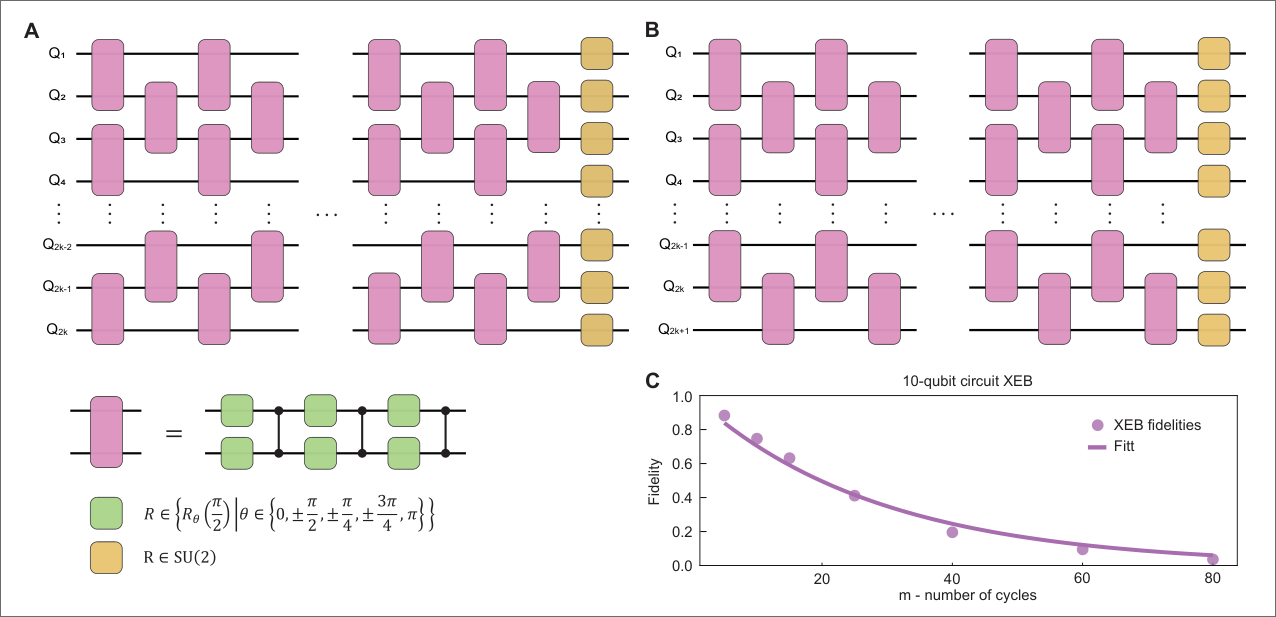
\includegraphics[scale=0.35]{inc/fig_05.png}
    \caption{
    Альтернативные квантовые схемы, используемые для бенчмаркинга CZ‑затворов,
    для чётного (A) и нечётного (B) числа кубитов. Зелёные квадраты обозначают
    случайно выбранные полу‑$\pi$‑повороты вокруг восьми осей, где $\theta$ —
    угол между осью поворота и осью $x$. Жёлтые квадраты обозначают затворы,
    случайно выбранные из $\mathrm{SU}(2)$. C, фиделити XEB как функция числа
    циклов затвора для случая с 10 кубитами. Ошибка цикла аппроксимирована
    значением около 3{,}45\,\%, причём каждый цикл содержит слой из 11
    однокубитных затворов, за которым в среднем следует слой из 4{,}5
    CZ‑затворов.
    }
    \label{fig:fig05}
\end{figure}

\subsection*{Процедура QAOA и сходимость}

QAOA может находить приближённое основное состояние гамильтониана путём
обновления параметров. Для QAOA с $p$ слоями участвуют $2p$ вариационных
параметров: $\boldsymbol{\gamma} = (\gamma_1, ..., \gamma_p)$ и
$\boldsymbol{\beta} = (\beta_1, ..., \beta_p)$. Основная задача квантового
процессора — многократно подготавливать следующую параметрическую волновую
функцию:

\begin{equation}
\lvert \gamma, \beta \rangle
      = e^{-i\beta_{p} H_{b}}
        e^{-i\gamma_{p} H_{c}}
        \dots
        e^{-i\beta_{1} H_{b}}
        e^{-i\gamma_{1} H_{c}}
        \lvert + \rangle^{n},
\end{equation}

\noindent где $H_b = \sum_{j=1}^{n} \sigma_x^j$ — это смешивающий гамильтониан. Это
состояние может быть подготовлено путём чередующегося применения унитарных
операторов $U(H_c, \gamma) = e^{-i\gamma H_c}$ и $U(H_b, \beta) = e^{-i\beta
H_b}$ с разными параметрами к состоянию равномерной суперпозиции $\lvert +
\rangle^{n}$. Классический оптимизатор используется для поиска оптимальных
параметров $(\boldsymbol{\gamma}^*, \boldsymbol{\beta}^*)$, минимизирующих
ожидаемое значение энергии проблемного гамильтониана:

\begin{equation}
E(\gamma, \beta)
      = \langle \gamma, \beta \lvert H_{c} \rvert \gamma, \beta \rangle
\end{equation}

Эта функция энергии может быть вычислена путём многократной подготовки волновой
функции $\lvert \boldsymbol{\gamma}, \boldsymbol{\beta} \rangle$ в квантовом
регистре и её измерения в вычислительном базисе. В результате получается
квантовое состояние $\lvert \boldsymbol{\gamma}^*, \boldsymbol{\beta}^*
\rangle$, соответствующее приближённому решению. Алгоритм графически
представлен на рис. \ref{fig:fig02}C.

Здесь мы кратко представим классический оптимизатор, используемый в QAOA во
время процедуры оптимизации параметров. Оптимизатор называется методом
модельного градиентного спуска (model gradient descent, MGD)~\cite{cite_48}. На
самом деле, можно рассмотреть и множество других классических алгоритмов
оптимизации, таких как метод симплекса Нелдера–Мида~\cite{cite_49},
квазиньютоновские методы~\cite{cite_50,cite_51}. Производительность этих
методов часто зависит от конкретной задачи. Показано как численно, так и
экспериментально, что модельный градиентный спуск работает хорошо для некоторых
вариационных квантовых анзацев~\cite{cite_11,cite_48}. Ключевая идея MGD —
использование модели для оценки градиента целевой функции, которая представляет
собой непрерывную поверхность или гиперповерхность. Для оценки градиента в
данной точке на поверхности случайным образом выбираются несколько близлежащих
точек и вычисляются значения целевой функции в этих точках. Затем квадратичная
модель аппроксимирует поверхность этих точек с помощью метода наименьших
квадратов. Градиент этой квадратичной модели используется в качестве замены
истинного градиента, и алгоритм спускается по соответствующему направлению.
Псевдокод приведён в алгоритме 3.

В нашем эксперименте метод MGD хорошо показал себя в трёх задачах факторизации.
Он сходится к локальному или глобальному оптимуму в пределах 10 шагов из
случайно выбранных начальных точек. При этом экспериментальные результаты
сходимости сопоставимы с теоретическими на текущем масштабе. Подробности о
траекториях сходимости приведены на рис. \ref{fig:fig06}.

\begin{figure}
    \centering
    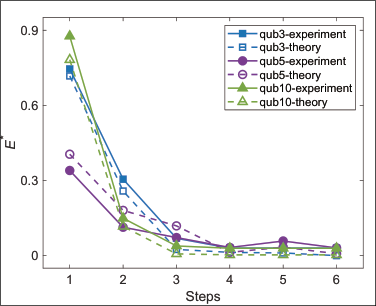
\includegraphics[scale=0.9]{inc/fig_06.png}
    \caption{
    Подробности о траекториях сходимости для трёх задач факторизации. Квадраты,
    кружки и треугольники соответствуют случаям с 3, 5 и 10 кубитами
    соответственно. Сплошные (пустые) символы обозначают экспериментальные
    (теоретические) результаты. По вертикальной оси отложено нормализованное
    значение энергетической функции $E^{*}$, а по горизонтальной оси — шаги
    вычислительной итерации.
    }
    \label{fig:fig06}
\end{figure}

\begin{algorithm}[htp!]
    \SetAlgoLined

    \KwData{начальная точка $x_0$, скорость обучения $\gamma$, радиус выборки $\delta$, количество точек $k$, показатель убывания скорости $\alpha$, постоянная устойчивости $A$, показатель убывания радиуса $\xi$, точность $\varepsilon$, максимальное число итераций $n$}
    \KwResult{оптимальное значение $x$}

    Инициализировать список $L$; \\
    $x \gets x_0$; \\
    $m \gets 0$; \\

    \While{число вычислений функции $+$ $k$ не превышает $n$}{
        Добавить кортеж $(x, f(x))$ в список $L$; \\
        $\delta' \gets \delta / (m + 1)^{\xi}$; \\
        Сэмплировать $k$ точек равномерно случайно из $\delta'$-окрестности $x$; пусть $S$ — полученное множество; \\
        \ForEach{$x' \in S$}{
            Добавить $(x', f(x'))$ в $L$;
        }

        Инициализировать список $L'$; \\
        \ForEach{кортеж $(x', y') \in L$}{
            \If{$\|x' - x\| < \delta'$}{
                Добавить $(x', y')$ в $L'$;
            }
        }

        Аппроксимировать квадратичную модель по точкам из $L'$ с помощью линейной регрессии с полиномиальными признаками; \\
        Пусть $g$ — градиент квадратичной модели в $x$; \\
        $\gamma' \gets \gamma / (m + 1 + A)^{\alpha}$; \\
        \If{$\gamma' \cdot \|g\| < \varepsilon$}{
            \Return $x$;
        }

        $x \gets x - \gamma' \cdot g$; \\
        $m \gets m + 1$;
    }

    \Return $x$;

    \caption{Алгоритм Model Gradient Descent}
    \label{alg:mgd}
\end{algorithm}


    \appendixsection{Постобработка: гладкие пары и линейные уравнения}

Ниже представлены другие гладкие соотношённые пары, полученные в примерах
факторизации чисел 1961, 48567227 и 261980999226229, как показано в следующих
списках. В первом столбце указаны порядковые номера гладких соотношённых пар
(sr-пар), а выражение $|u - vN|$ представлено в виде разложения по
соответствующему простому базису. В случае с 3 кубитами мы приводим 20
независимых гладких соотношённых пар, и соответствующая булева матрица состоит
из 20 векторов размерности 16. Следовательно, среди них обязательно найдётся
группа линейно зависимых векторов, то есть система линейных уравнений имеет как
минимум одно решение.

\subsection*{Случай с 3 кубитами}

В таблице Е.9 приведён список булевых векторов, соответствующих показателям
простого базиса, составленного из $u / (u - vN)$. Можно заметить, что четвёртый
вектор является нулевым, что само по себе представляет собой вектор линейной
зависимости. 10-й и 17-й векторы, а также 5-й и 16-й — это две группы линейно
зависимых векторов. Другие линейно зависимые векторы необходимо определить,
решая систему линейных уравнений. Каждая такая группа линейных зависимостей
будет соответствовать квадратичному сравнению вида $X^2 \equiv Y^2 \pmod{N}$. С
высокой вероятностью факторизация числа $N$ может быть получена с помощью этого
сравнения. Ниже мы приводим подробности факторизации $N = 1961$ с
использованием конкретных гладких соотношённых пар.

Согласно приведённому выше обсуждению, из указанных гладких соотношённых пар
можно найти решения системы линейных уравнений, например:

\textbf{Пример 1:} 4-я пара, где $u = 34 \cdot 5^2$, $v = 1$, $|u - vN| = 26$,
что даёт квадратичное сравнение: $(9 \cdot 5)^2 - 8^2 = N$. Тогда: $p = \gcd(45
+ 8, N) = 53, \quad q = \gcd(45 - 8, N) = 37$.

\textbf{Пример 2:} 9-я пара, где $u = 26 \cdot 5^2$, $v = 1$, $|u - vN| =
19^2$, $(8 \cdot 5)^2 + 19^2 = N$, и, согласно методу факторизации Гаусса, это
приведёт к паре множителей:
\begin{equation}
p = x^2 + y^2, \quad q = a^2 + b^2.
\end{equation}

Далее:
\begin{equation}
\left\{
\begin{aligned}
|ax - by| &= 40,\\
|bx + ay| &= 19,
\end{aligned}
\right.
\quad \text{или} \quad
\left\{
\begin{aligned}
|ax - by| &= 19,\\
|bx + ay| &= 40.
\end{aligned}
\right.
\end{equation}

Решая уравнения, получаем: $a = 1$, $b = 6$, $x = 2$, $y = 7$. Подставляя в
уравнение (Е.55), получаем $p = 53$, $q = 37$. Или: $a = 2$, $b = 7$, $x = 6$,
$y = -1$, тогда $p = 37$, $q = 53$.

\textbf{Пример 3:} Комбинация 10-й и 17-й пары даёт:
\begin{equation}
(2 \cdot 5^2 \cdot 2^2 \cdot 3^3)^2 \equiv (7 \cdot 11 \cdot 13)^2 \pmod{1961}.
\end{equation}
Отсюда:

\begin{equation}
p = \gcd(5400 + 1001, 1961) = 37,
\end{equation}
\begin{equation}
q = \gcd(5400 - 1001, 1961) = 53.
\end{equation}

\textbf{Пример 4:} Комбинация 5-й и 16-й пары:
\begin{equation}
2^5 \cdot 5^2 \cdot 3 \cdot 5^4 \equiv 2 \cdot 4^3 \cdot 3^3 \cdot 4^3 \pmod{1961},
\end{equation}
то есть:
\begin{equation}
(2^2 \cdot 5^3)^2 \equiv (4^3 \cdot 3)^2 \pmod{1961}.
\end{equation}

Следовательно:
\begin{equation}
p = \gcd(500 + 129, 1961) = 37,
\end{equation}
\begin{equation}
q = \gcd(500 - 129, 1961) = 53.
\end{equation}

Кроме того, простые множители также могут быть найдены с помощью решений
линейных уравнений для других соотношений, которые здесь не приводятся.

\begin{table}[H]
\centering
\caption{
    Булевы экспоненциальные векторы, соответствующие гладким соотношённым
    парам. Первый столбец представляет собой порядковый номер гладкой
    соотношённой пары $(u, v)$. Второй столбец — это знак, который указывает на
    положительность или отрицательность выражения $u / (u - vN)$. Столбцы с
    третьего по семнадцатый представляют булевы показатели для первых 15
    простых чисел базиса соответственно.
}
\begin{tabular}{c|c|*{15}{c}}
\hline
\hline
\textbf{sn} & \textbf{sign} & $p_1$ & $p_2$ & $p_3$ & $p_4$ & $p_5$ & $p_6$ & $p_7$ & $p_8$ & $p_9$ & $p_{10}$ & $p_{11}$ & $p_{12}$ & $p_{13}$ & $p_{14}$ & $p_{15}$ \\
\hline
1 & 1 & 1 & 1 & 0 & 0 & 0 & 0 & 1 & 0 & 0 & 0 & 0 & 0 & 0 & 0 & 0 \\
2 & 0 & 0 & 1 & 0 & 1 & 0 & 0 & 1 & 0 & 0 & 0 & 0 & 0 & 0 & 0 & 0 \\
3 & 1 & 1 & 1 & 0 & 0 & 0 & 0 & 0 & 0 & 0 & 0 & 0 & 1 & 0 & 1 & 0 \\
4 & 0 & 0 & 0 & 0 & 0 & 0 & 0 & 0 & 0 & 0 & 0 & 0 & 0 & 0 & 0 & 0 \\
5 & 1 & 1 & 1 & 0 & 0 & 0 & 0 & 0 & 0 & 0 & 0 & 0 & 0 & 0 & 1 & 0 \\
6 & 1 & 1 & 0 & 1 & 0 & 1 & 0 & 0 & 0 & 1 & 0 & 0 & 0 & 0 & 0 & 0 \\
7 & 0 & 1 & 0 & 1 & 0 & 0 & 0 & 0 & 0 & 0 & 0 & 0 & 0 & 0 & 0 & 0 \\
8 & 1 & 0 & 1 & 0 & 0 & 1 & 0 & 0 & 0 & 1 & 0 & 0 & 0 & 0 & 0 & 0 \\
9 & 1 & 0 & 1 & 0 & 0 & 0 & 1 & 0 & 0 & 0 & 0 & 0 & 0 & 0 & 0 & 0 \\
10 & 1 & 0 & 0 & 1 & 0 & 0 & 0 & 0 & 0 & 0 & 0 & 0 & 0 & 0 & 0 & 0 \\
11 & 1 & 1 & 1 & 0 & 1 & 0 & 1 & 0 & 0 & 0 & 0 & 0 & 0 & 0 & 0 & 1 \\
12 & 1 & 0 & 0 & 1 & 1 & 0 & 0 & 1 & 0 & 0 & 0 & 0 & 0 & 0 & 0 & 0 \\
13 & 1 & 0 & 1 & 0 & 0 & 0 & 0 & 0 & 1 & 0 & 0 & 0 & 0 & 0 & 0 & 0 \\
14 & 1 & 1 & 0 & 0 & 0 & 0 & 0 & 0 & 0 & 0 & 0 & 0 & 0 & 0 & 0 & 0 \\
15 & 1 & 0 & 1 & 0 & 0 & 0 & 0 & 1 & 0 & 1 & 0 & 0 & 0 & 0 & 1 & 0 \\
16 & 1 & 1 & 1 & 0 & 0 & 0 & 0 & 0 & 0 & 0 & 0 & 0 & 1 & 0 & 1 & 0 \\
17 & 0 & 0 & 0 & 0 & 0 & 0 & 0 & 0 & 0 & 0 & 0 & 0 & 0 & 0 & 0 & 0 \\
18 & 0 & 0 & 1 & 0 & 1 & 0 & 0 & 0 & 0 & 0 & 0 & 0 & 1 & 0 & 0 & 1 \\
19 & 0 & 1 & 0 & 1 & 0 & 0 & 1 & 0 & 0 & 0 & 0 & 0 & 0 & 0 & 0 & 0 \\
20 & 0 & 0 & 1 & 0 & 1 & 0 & 0 & 1 & 0 & 0 & 0 & 0 & 1 & 0 & 1 & 0 \\
\hline
\hline
\end{tabular}
\end{table}

\subsection*{Случай с 5 кубитами}

В случае с 5 кубитами мы приводим 55 независимых гладких соотношённых пар в
следующем списке. Соответствующая булева матрица содержит 55 векторов
размерности 51 (50 измерений для простого базиса и 1 измерение для знака).
Аналогично, среди них обязательно найдётся группа линейно зависимых векторов.

Из-за высокой размерности векторов, соответствующих случаю с 5 кубитами, мы
приводим только одно решение системы линейных уравнений:

\begin{equation}
\begin{aligned}
x = (&0, 0, 0, 0, 0, 0, 0, 0, 1, 0, 0, 1, 1, 0, 0, 0, 1, 0, 0, \\
&1, 1, 0, 0, 1, 0, 0, 0, 1, 0, 1, 0, 0, 0, 0, 0, 0, 0, \\
&0, 0, 0, 0, 0, 0, 1, 1, 1, 0, 0, 0, 0).
\end{aligned}
\end{equation}

Соответствующее решение для квадратичного сравнения:
\begin{equation}
\begin{aligned}
X &= 639232456435359657331994419097900390625, \\
Y &= 12136572734325633629343926054845304.
\end{aligned}
\end{equation}

Нетрудно проверить, что данное решение удовлетворяет уравнению:

\begin{equation}
X^2 \equiv Y^2 \pmod{N}
\end{equation}

Кроме того, имеем:

\begin{equation}
\begin{aligned}
p &= \gcd(X + Y, N) \\
  &= \gcd(639232456435359657331994419097900390625 + \\
  &\quad \ 12136572734325633629343926054845304, \,48567227) \\
  &= 7919, \\
q &= \gcd(X - Y, N) \\
  &= \gcd(639232456435359657331994419097900390625 - \\
  &\quad \ 12136572734325633629343926054845304, \,48567227) \\
  &= 6133.
\end{aligned}
\end{equation}

В результате мы получаем разложение числа на множители:
$N = 48567227 = 7919 \times 6133$.

\subsection*{Случай с 10 кубитами}

В случае с 10 кубитами мы приводим 221 независимую гладкую пару в
Дополнительных материалах. Соответствующая булева матрица содержит 221 вектор
размерности 201 (200 измерений для простого базиса и 1 измерение для знака). Мы
приводим одно решение системы линейных уравнений:

\begin{equation}
\begin{aligned}
x = (&1, 0, 0, 0, 0, 0, 0, 0, 0, 0, 0, 0, 0, 0, 0, 0, 0, 0, 0, 0, 0, 0, 0, 0, 0, \\
     &0, 0, 0, 0, 0, 0, 0, 0, 0, 0, 0, 0, 0, 0, 0, 0, 0, 0, 0, 0, 0, 0, 0, 1, \\
     &1, 1, 0, 0, 0, 1, 0, 0, 0, 0, 1, 0, 0, 0, 0, 1, 1, 0, 0, 0, 0, 1, 0, 1, \\
     &1, 0, 1, 1, 0, 0, 1, 0, 0, 0, 1, 1, 1, 0, 0, 0, 1, 0, 1, 1, 1, 0, 1, 0, \\
     &1, 0, 0, 1, 0, 0, 0, 0, 1, 1, 1, 1, 0, 1, 1, 0, 1, 0, 1, 0, 0, 1, 0, 0, \\
     &1, 1, 0, 0, 0, 1, 1, 0, 0, 0, 0, 1, 0, 0, 1, 1, 1, 0, 1, 0, 0, 0, 0, 1, \\
     &0, 0, 1, 0, 1, 1, 1, 1, 0, 1, 0, 0, 0, 0, 1, 0, 1, 0, 0).
\end{aligned}
\end{equation}

Соответствующее решение для квадратичного сравнения представлено в уравнении:
\begin{equation}
\begin{aligned}
X = &75695763106501556705305764502754936587819598184067351577 \\
    &43303250785633285956794230102519018501335269995854539435 \\
    &01610097294132617819824833811012145914436530877754829641 \\
    &771815233949422940291369528064063220752769498277701462410 \\
    &831032646021654929699823769255863972607946356507092437520 \\
    &628983005772258943590442184281264255447072655152539925075 \\
    &228232905527827902441430959155400833286647355489098701203 \\
    &6652660975430964340161981191012698547957753245615400642156 \\
    &6009521484375000000000000000000000000000000000000000000, \\ \\
Y = &89703025676439146996343189305085999464349858249769290536 \\
    &39263868715312151470596839682183291916841767330486102677 \\
    &2500921420533610666859894934306516222448335298649730188 \\
    &139419712140836303477738769684013638969809410021181628 \\
    &148458466644646455709975881417989619205326153001893986 \\
    &178123643916398321728850997506608105566537622917582126 \\
    &731375145833485980298044011134125822403913885046671262 \\
    &19915873471668113404162973340975659170623801.
\end{aligned}
\end{equation}

Нетрудно проверить, что данное решение удовлетворяет следующему уравнению:
\begin{equation}
X^2 \equiv Y^2 \pmod{N}
\end{equation}

Кроме того, имеем:
\begin{equation}
\begin{aligned}
p &= \gcd(X + Y, N) = 15538213, \\
q &= \gcd(X - Y, N) = 16860433.
\end{aligned}
\end{equation}

В результате мы получаем разложение на множители:
\begin{equation}
N = 261980999226229 = 15538213 \times 16860433.
\end{equation}


    \appendixsection{Исследование квантового преимущества}

В этой части мы численно исследуем преимущество квантового оптимизатора по
сравнению с алгоритмом Бабая. Рассматриваемый критерий измерения — это качество
коротких векторов для задачи ближайшего вектора (CVP). Качество короткого
вектора положительно коррелирует с эффективностью получения гладких
соотношённых пар в более эффективном методе факторизации Шнорра. Поскольку в
настоящее время оценка аналитической сложности алгоритма QAOA остаётся открытым
вопросом, в данном обсуждении предполагается, что процедура QAOA способна
находить оптимальное решение задачи оптимизации за ограниченное время. Здесь мы
используем параметр относительного расстояния $r$ для измерения длины вектора
вместо евклидовой нормы или квадратной нормы. Параметр определяется следующим
образом:

\begin{equation}
r = \frac{\lVert \mathbf{b} - \mathbf{t} \rVert^2}{\det(\mathbf{B}'_{n,c})^{\frac{2}{n}}},
\end{equation}

где $B'_{n,c} = [B_{n,c},\, N c]$. Этот параметр использует $2/n$‑степень
определителя расширенной решётки $B'_{n,c}$ для измерения относительной длины
короткого вектора $b - t$, что позволяет в определённой степени уменьшить
влияние различий в определителе решёток на качество коротких векторов.

\subsection*{Результаты на случайных выборках}

Сначала мы исследуем производительность квантового оптимизатора и классического
алгоритма Бабая на случайных выборках задачи CVP. Здесь мы генерируем 50
случайных примеров CVP (решётка и целевой вектор) при условиях размерности
решётки $n = 7$, точности $c = 10$ и $n = 10$, $c = 7$ соответственно. Для
каждой случайной выборки определитель решётки и целевой вектор остаются
одинаковыми — меняются только элементы главной диагонали решётки, которые
случайным образом переставляются. Результаты представлены на рис.
\ref{fig:fig08}. По горизонтальной оси отложены случайные выборки, по
вертикальной — относительное качество $r$ результирующего вектора. Синие
(жёлтые) столбцы представляют результаты классического алгоритма Бабая
(квантовой оптимизации). Как видно на графике, результаты, полученные с помощью
квантовой оптимизации, не хуже классических, а во многих случаях существенно
лучше, то есть получены более короткие векторы.

\begin{figure}
    \centering
    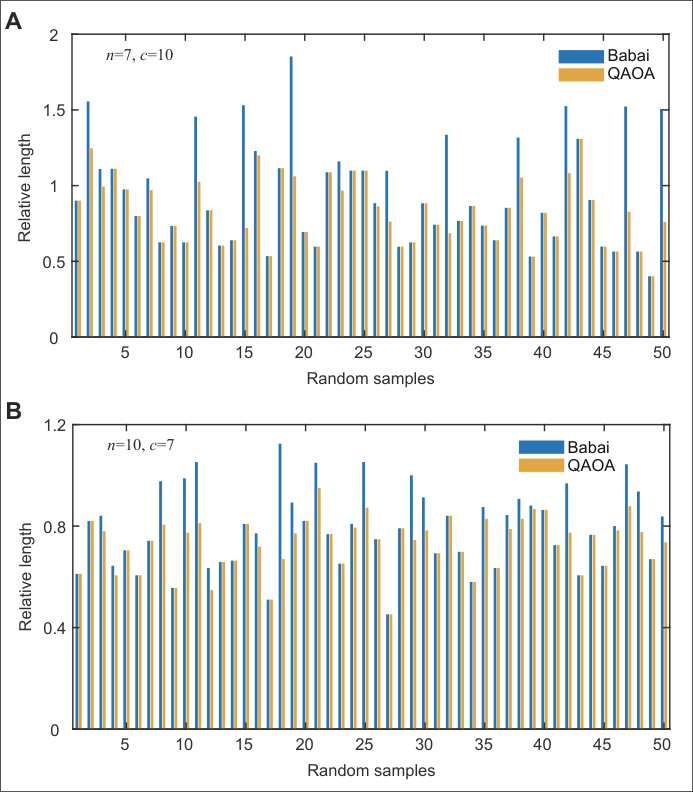
\includegraphics[scale=0.6]{inc/fig_08.png}
    \caption{
    Производительность на случайных выборках для квантового оптимизатора (QAOA)
    по сравнению с алгоритмом Бабая. A (B) — результаты для 50 случайных
    примеров задачи CVP при условиях $n = 7$, $c = 10$ ($n = 10$, $c = 7$).
    Жёлтые (синие) столбцы представляют результаты квантового оптимизатора
    (классического алгоритма Бабая). Можно наблюдать, что в ряде случаев
    результаты квантовой оптимизации превосходят классические.
    }
    \label{fig:fig08}
\end{figure}

\subsection*{Квантовое преимущество и точность решётки}

Мы дополнительно исследуем преимущество квантового оптимизатора при увеличении
параметра точности $c$ решётки. На рис. \ref{fig:fig09}A представлены численные
результаты при увеличении параметра $c$ от 5 до 14 для размерностей решётки $n
= 12$ и $n = 14$ соответственно. Результаты усреднены по 40 случайно
сгенерированным примерам задачи CVP для каждого набора параметров $\{n, c\}$.
Символы в виде кружков (треугольников) соответствуют результатам при $n = 12$
($n = 14$). Сплошные (пустые) символы обозначают результаты квантового
(классического) алгоритма. Погрешности отображают доверительный интервал при
стандартном отклонении, равном единице.

В обоих случаях, при $n = 12$ и $n = 14$, после квантовой оптимизации
получаются более короткие векторы. Рассматривая случай $n = 14$ в качестве
примера, можно увидеть, что разрыв в качестве между результатами алгоритма
Бабая и квантового алгоритма постепенно увеличивается с ростом параметра $c$.
Это указывает на то, что качество вектора после квантовой оптимизации в среднем
выше, чем у алгоритма Бабая, при увеличении определителя решётки.

Кроме того, на рис. \ref{fig:fig09}B приведена доля выборок, где квантовая
оптимизация дала преимущество, относительно всех 40 случайных примеров. Эти
доли показаны синими и оранжевыми столбцами для случаев $n = 12$ и $n = 14$
соответственно. Мы обнаружили, что для $n = 12$ доля квантового преимущества
составляет примерно 0{,}5, а для $n = 14$ она увеличивается до 0{,}65.
Результаты свидетельствуют о том, что квантовое преимущество становится более
заметным при увеличении размерности решётки. Эти результаты будут дополнительно
подтверждены в следующем разделе.

\subsection*{Квантовое преимущество и размерность решётки}

Здесь мы исследуем зависимость преимущества квантового оптимизатора от
размерности решётки до $n = 14$. Для каждой размерности $n$ результаты
усреднены по 40 случайным выборкам при $c = n$. Как показано на рис.
\ref{fig:fig10}A, качество вектора после квантовой оптимизации в среднем выше,
чем при использовании классического алгоритма Бабая.
\begin{figure}
    \centering
    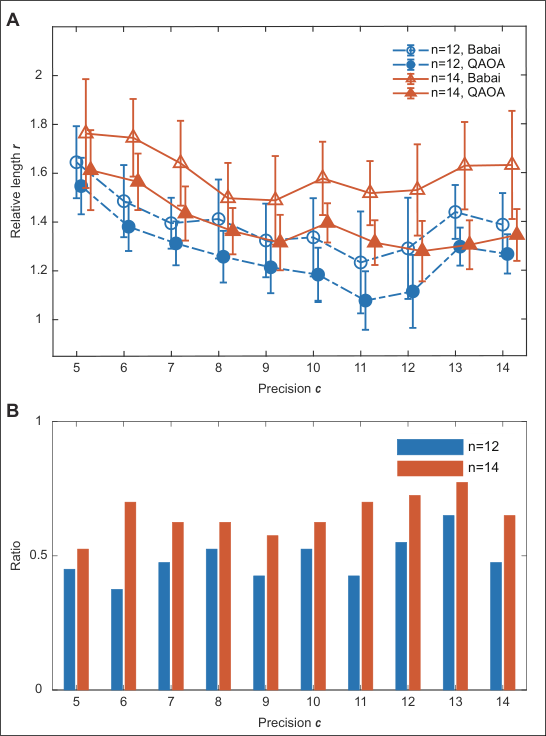
\includegraphics[scale=0.6]{inc/fig_09.png}
    \caption{
    Производительность квантового оптимизатора при увеличении точности решётки.
    A: Относительные длины для квантовых и классических методов. По
    горизонтальной оси отложен параметр точности $c$, положительно
    коррелирующий с определителем решётки. B: Доля квантового преимущества для
    40 случайных выборок, синие (оранжевые) столбцы для случая $n = 12$ ($n =
    14$). На графике видно, что в среднем квантовая оптимизация даёт лучшие
    результаты, особенно при больших значениях определителя (связанного с $c$).
    }
    \label{fig:fig09}
\end{figure}

Иначе говоря, с помощью квантовой оптимизации можно найти более короткий
вектор. Разрыв в качестве между квантовыми и классическими результатами
становится более заметным с увеличением размерности решётки, что означает, что
преимущество квантового метода возрастает в более крупных системах. Также мы
подсчитали долю квантового преимущества среди 40 случайных выборок,
представленных на рис. \ref{fig:fig10}B. Эта доля возрастает с увеличением
размерности, что согласуется с различием тенденций на графиках качества
векторов на рис. \ref{fig:fig10}A. Оба результата указывают на то, что
преимущества квантовых методов будут становиться всё более очевидными с ростом
размерности решётки.

\begin{figure}
    \centering
    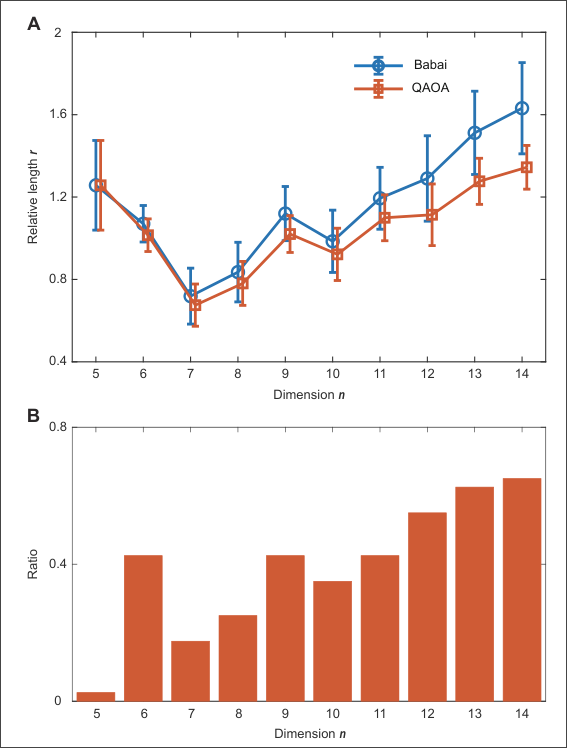
\includegraphics[scale=0.6]{inc/fig_10.png}
    \caption{
    Производительность квантового оптимизатора при увеличении размерности
    решётки. A: Относительная длина векторов для квантового и классического
    методов. По горизонтальной оси отложена размерность решётки $n$. Результаты
    усреднены по 40 случайным выборкам при $c = n$. Погрешности отображают
    доверительный интервал при стандартном отклонении, равном единице. B: Доля
    квантового преимущества среди 40 случайных выборок. Можно заметить, что
    разрыв в относительном расстоянии между квантовыми и классическими
    результатами увеличивается с ростом размерности решётки.
    }
    \label{fig:fig10}
\end{figure}

    \appendixsection{Оценка ресурсов для RSA-2048}

\subsection*{Введение}

Сколько квантовых ресурсов требуется для факторизации 2048-битного RSA-числа? В
этом разделе мы сосредотачиваемся на конкретных квантовых ресурсах, необходимых
для факторизации 2048-битного RSA-числа на основе алгоритма SQIF.
Рассматриваемые квантовые ресурсы в основном включают количество физических
кубитов и глубину схемы QAOA с одним слоем. Обычно квантовые схемы не могут
быть непосредственно выполнены на квантовых вычислительных устройствах,
поскольку при их разработке не учитываются особенности связности кубитов или
топологии реальных физических систем. Процесс выполнения часто требует
дополнительных квантовых ресурсов, таких как вспомогательные (ancilla) кубиты и
увеличение глубины схемы. Мы обсуждаем необходимые квантовые ресурсы для
факторизации реальных RSA-чисел в терминах трёх типов топологий: полной
графовой топологии ($K_n$), двумерной решётки (2DSL) и одномерной цепочки
(LNN). Мы демонстрируем с использованием конкретных схем, что процесс внедрения
(embedding) не требует дополнительных кубитов. Более того, глубина схемы QAOA с
одним слоем линейно зависит от размерности $n$ квантовой системы для всех трёх
топологий. Таким образом, для факторизации целых чисел с использованием
алгоритма SQIF мы потребляем сублинейное количество квантовых ресурсов. В
качестве примера рассмотрим RSA-2048. Необходимое количество кубитов
оценивается как $n = \frac{2 \cdot 2048}{\log 2048} \approx 372$. Глубина
квантовой схемы QAOA с одним слоем составляет 1118 для топологии $K_n$, 1139
для топологии 2DSL и 1490 для самой простой топологии LNN. Эти значения
достижимы для NISQ-устройств в ближайшем будущем или даже уже сегодня.

\subsection*{Описание проблемы}

Сначала рассмотрим построение гамильтониана $H_c$. Используя правила
однокубитного кодирования, соответствующий гамильтониан $H_c$ может быть
представлен как двумерная изинговская модель следующего вида:

\begin{equation}
H_c = \sum_{i=1}^{n} h_i \sigma_z^i + \sum_{i,j=1}^{n} J_{i,j} \sigma_z^i \sigma_z^j,
\end{equation}

где параметры $h_i$, $J_{i,j}$ определяются коэффициентами линейных и
квадратичных членов задачи квадратичной безусловной бинарной оптимизации
(QUBO). Символ суммы в правой части второго выражения пробегает все комбинации
индексов. Если рассматривать каждый квадратичный член как ребро в
неориентированном графе, то все ZZ-члены $\{\sigma_i^z \sigma_j^z\}_{i<j}$
формируют полный граф порядка $n$, то есть граф $K_n$. Иначе говоря, топология
связности логических кубитов — это граф $K_n$. В качестве примеров можно
рассмотреть случаи с 3 кубитами и 5 кубитами, приведённые в основном тексте:
топология кубитов проблемного гамильтониана представляет собой соответственно
полный граф порядка 3 и 5, как показано на рис. \ref{fig:fig11}A и B.

\begin{figure}
    \centering
    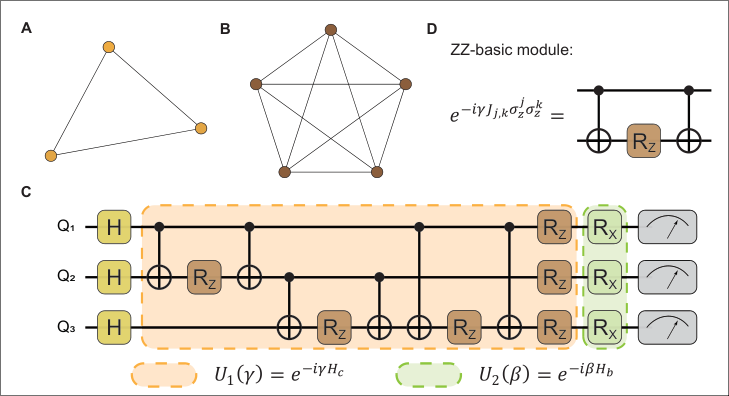
\includegraphics[scale=0.6]{inc/fig_11.png}
    \caption{
    Связность кубитов и типичная квантовая схема QAOA. A — топология связности
    кубитов для случая с 3 кубитами, представляющая собой граф $K_3$. B —
    случай с 5 кубитами, соответствующий графу $K_5$. C — типичная квантовая
    схема QAOA с одним слоем для гамильтониана QUBO на 3 кубитах. Она в
    основном состоит из двух операторов: $U_1(\gamma)$ и $U_2(\beta)$,
    соответствующих операторам эволюции проблемного гамильтониана $H_c$ и
    смешивающего гамильтониана $H_b$ соответственно. D — базовый модуль ZZ. Он
    состоит из двух CNOT-затворов и одного однокубитного вращения $R_z$,
    расположенных по схеме «бутерброда».
    }
    \label{fig:fig11}
\end{figure}

Типичная схема QAOA для гамильтониана типа $K_n$ показана на рис.
\ref{fig:fig11}C. В квантовой схеме однослойной итерации QAOA участвуют два
типа унитарных операторов. $U_1(\gamma)$ — оператор эволюции проблемного
гамильтониана $H_c$, а $U_2(\beta)$ — оператор эволюции смешивающего
гамильтониана $H_b$, состоящего из однокубитных вращений вокруг оси $x$.
Оператор $U_1(\gamma)$ можно реализовать с помощью однокубитных вращений $R_z$
и двухкубитных блоков, соответствующих локальным (линейным) членам и ZZ-членам
гамильтониана $H_c$. Основное внимание мы уделяем двухкубитным блокам, которые
определяются следующим образом:

\begin{equation}
\mathrm{ZZ}_{j,k}(\gamma) = e^{-i \gamma J_{j,k} \sigma_z^j \sigma_z^k}.
\end{equation}

Унитар $\text{ZZ}_{j,k}(\gamma)$ можно реализовать с помощью комбинации двух
CNOT-затворов и одного $R_z$-затвора, образующих «бутерброд», как показано на
рис. \ref{fig:fig11}D. В дальнейших обсуждениях мы будем рассматривать такую
комбинацию затворов как базовый модуль глубины 3 без учёта его компиляции в
конкретной физической системе. Физическая система, как правило, компилирует
этот модуль на основе своей нативной универсальной системы квантовых затворов,
и это обычно приводит к добавлению не более чем $O(1)$ дополнительных операций
и увеличению глубины схемы.

Так как глубина схемы для однокубитных операций в $U_1(\gamma)$ и $U_2(\beta)$
не превышает 2 в физической реализации, мы не будем их далее обсуждать. Мы
сосредотачиваемся на задаче внедрения квадратичных членов из $U_1(\gamma)$ в
физическую систему. В частности, мы оцениваем накладные затраты по числу
кубитов и глубине схемы после внедрения группы ZZ-членов, образующих схему типа
$K_n$. В дальнейшем эта задача будет называться задачей внедрения типа $K_n$
(Kn-type embedding problem).

\subsection*{Глубина схемы при топологии полного графа}

Сначала рассмотрим идеальный случай, при котором любые два кубита могут
напрямую взаимодействовать. Иначе говоря, топология связности кубитов в
физической системе представляет собой полный граф. В этом сценарии задача
внедрения схемы типа $K_n$ не требует дополнительных кубитов или квантовых
SWAP-затворов. Следовательно, глубина квантовой схемы может быть
минимизирована.

Полный граф $K_n$ содержит $n(n - 1)/2$ рёбер, что означает, что схема QAOA
содержит $O(n^2)$ базовых модулей ZZ. Глубина однослойной схемы QAOA без
оптимизации составляет $O(n^2)$. Поскольку ZZ-члены в операторе $U_1(\gamma)$
коммутируют между собой, мы можем произвольно переставлять порядок двухкубитных
взаимодействий, чтобы минимизировать глубину схемы.

Здесь мы представляем схему оптимизации, основанную на теории максимального
паросочетания в неориентированном графе, которая позволяет уменьшить глубину
схемы до $O(n)$. Эта схема является оптимальной, если рассматривать ZZ-член как
базовый модуль.

\textbf{Определение 2}. Паросочетание и максимальное паросочетание. Обозначим
неориентированный граф как $G(V, E)$ и пусть $M \subseteq E(G)$ — подмножество
рёбер, такое что для всех пар $(e_i, e_j) \in M$ рёбра $e_i$ и $e_j$ не смежны
в $G$. То есть рёбра в $M$ не имеют общих вершин. Тогда $M$ называется
паросочетанием в графе $G$. Для каждого ребра $e = (u, v)$ в паросочетании $M$,
говорят, что ребро $e$ и вершины $u$, $v$ покрыты паросочетанием $M$. Каждая
вершина в графе либо не покрыта $M$, либо покрыта ровно одним ребром из $M$.
Если не существует другого паросочетания $M'$ в $G$, такого что $|M'| > |M|$,
то $M$ называется максимальным паросочетанием в $G$. Если каждая вершина в $G$
покрыта паросочетанием $M$, то $M$ называется совершенным паросочетанием в $G$.

Согласно определению, совершенное паросочетание обязательно является
максимальным. Количество максимальных паросочетаний в полном графе определяется
следующей леммой.

\textbf{Лемма 3} (Максимальное паросочетание в полном графе) Существует $2n -
1$ совершенных паросочетаний без повторяющихся рёбер в полном графе чётного
порядка $K_{2n}$. Аналогично, существует $2n - 1$ максимальных паросочетаний
без повторяющихся рёбер в полном графе нечётного порядка $K_{2n - 1}$.

\textit{Доказательство.} Для полного графа чётного порядка $K_{2n}$ расположим
вершины $v_1, v_2, \dots, v_{2n-1}$ по окружности в виде $(2n - 1)$‑угольника и
добавим вершину $v_{2n}$ в центр. Выберем произвольную вершину $v_i$, где $1
\leq i \leq 2n - 1$, и построим паросочетание $M_i$, включающее ребро $(v_i,
v_{2n})$ и все рёбра, перпендикулярные ему. Легко доказать, что $M_i$ —
совершенное паросочетание для любого $i$, и ни одно ребро не повторяется между
$M_i$ и $M_j$, если $i \ne j$. Таким образом, в полном графе $K_{2n}$
существует $2n - 1$ совершенных паросочетаний без повторений. Так как в графе
$K_{2n}$ всего $n(2n - 1)$ различных рёбер, и $2n - 1$ совершенных
паросочетаний уже покрывают их без повторений, других возможных неповторяющихся
паросочетаний не существует. Для случая нечётного полного графа $K_{2n - 1}$
добавим вспомогательную вершину $v_{2n}$, тем самым превратив задачу в случай
чётного порядка. Затем в каждом совершенном паросочетании удалим ребро $(v_i,
v_{2n})$. В результате получим $2n - 1$ максимальных паросочетаний для
нечётного случая. Это завершает доказательство.

\textbf{Утверждение 3}

Если связность кубитов в физической системе представляет собой полный граф, то
гамильтониан типа $K_n$ может быть внедрён без дополнительных кубитов, а
глубина внедрённой квантовой схемы составляет $O(n)$.

\textit{Доказательство.} Согласно определению паросочетания (см. Определение
2), рёбра в одном паросочетании не имеют общих вершин. Следовательно,
соответствующие двухкубитные взаимодействия можно выполнять одновременно и
параллельно. Предположим, что каждый ZZ-член компилируется с использованием
базового модуля ZZ (см. рис.~S7D), тогда глубина схемы для одного паросочетания
равна 3. Согласно Лемме 3, если $n$ чётно, то в полном графе $K_n$ существует
$n - 1$ неповторяющихся совершенных паросочетаний, покрывающих все рёбра.
Значит, можно построить квантовую схему из $n - 1$ слоёв, где каждый слой
содержит $n/2$ модулей ZZ, выполняемых параллельно. Общая глубина схемы
составит $3(n - 1)$. Если $n$ нечётно, то по Лемме 3 в полном графе $K_n$
существует $n$ максимальных паросочетаний без повторяющихся рёбер. Каждое такое
паросочетание содержит $(n - 1)/2$ рёбер, и все вместе они покрывают все рёбра
графа $K_n$. Значит, можно построить квантовую схему из $n$ слоёв, каждый из
которых выполняет $(n - 1)/2$ двухкубитных операций параллельно. Общая глубина
схемы составляет $3n$. Таким образом, схема типа $K_n$ может быть реализована
без дополнительных кубитов, а глубина внедрённой квантовой схемы составляет
$O(n)$. Доказательство завершено.

Доказательство Леммы 3 предоставляет точную конструкцию каждого совершенного
паросочетания в полном графе $K_n$, а значит — и точную схему построения
внедрённой квантовой схемы с глубиной $O(n)$. Схема оптимальна, если
рассматривать ZZ-члены в качестве базового модуля. В таком случае количество
ZZ-операций в каждом слое максимально, то есть достигается наивысшая степень
параллелизма. Поскольку все максимальные (совершенные) паросочетания покрывают
все рёбра без повторений, схема является оптимальной.

Связность кубитов — это ценный ресурс в устройствах NISQ. Как правило,
построение полносвязной топологии в масштабируемых квантовых системах
затруднено. Тем не менее, она достижима в некоторых особых системах, таких как
ионные ловушки~\cite{cite_52}, оптические квантовые системы и системы с большой
квантовой памятью~\cite{cite_15}.

\subsection*{Глубина схемы при линейной и решётчатой топологиях}

Линейная цепочка (linear chain) — одна из самых распространённых топологий,
которая относительно легко реализуется в реальных квантовых системах. Эта
топология, также известная как архитектура линейного ближайшего соседа (LNN),
предполагает расположение кубитов на линии с возможностью взаимодействия только
между соседними кубитами. В этом разделе мы рассматриваем ресурсы по числу
квантовых затворов и глубине схемы при внедрении гамильтониана типа $K_n$ в
одномерную систему LNN. Результаты для двумерной решётки (lattice system) можно
сформулировать как следствие.

Задача внедрения произвольных топологий гамильтонианов в LNN широко
исследуется~\cite{cite_53,cite_54,cite_55,cite_56,cite_57,cite_58,cite_59}, и
уже существуют зрелые методы. В 2007 году Донни Чеунг и др.~\cite{cite_55}
исследовали накладные расходы при преобразованиях между различными топологиями
на основе графовых моделей. Они указали, что отображение произвольной схемы в
LNN требует не более $O(n)$ дополнительной глубины на основе параллельной
сортировки. Однако конкретная схема преобразования гамильтониана типа $K_n$ в
LNN ими не приводится. В 2009 году Юити Хирата предложил эффективный метод
отображения произвольных квантовых схем в LNN на основе идеи пузырьковой
сортировки~\cite{cite_56}. В 2021 году исследователи из Google применили
параллельную пузырьковую сортировку для выполнения внедрения из $K_{17}$ в LNN
и провели соответствующие эксперименты на сверхпроводниковом квантовом
процессоре Sycamore~\cite{cite_11}. В целом, отображение $K_n$ в LNN требует
$O(n^2)$ операций SWAP и $O(n)$ дополнительной глубины схемы при использовании
параллельной пузырьковой сортировки. Ниже мы приведём независимое
доказательство этого результата на основе параллельного пузырькового алгоритма.

Чтобы внедрить полный граф $K_n$ в LNN, необходимо выполнять дополнительные
SWAP-операции для перестановки (или сортировки) кубитов в нужном порядке.
Минимизация числа SWAP-затворов является ключевой задачей. Согласно
работе~\cite{cite_56}, сеть SWAP-операций пузырьковой сортировки оптимальна для
этой цели. Следовательно, справедлива следующая лемма.

\textbf{Лемма 4.} Пусть $x_1, x_2, \dots, x_n$ — начальный порядок $n$ кубитов
в архитектуре LNN. Рассмотрим перестановку, изменяющую порядок на $x_{j_1},
x_{j_2}, \dots, x_{j_n}$. Минимальное число необходимых SWAP-затворов
эквивалентно числу операций обмена в алгоритме пузырьковой сортировки.

Лемма 4 показывает, что пузырьковая сортировка является оптимальной для
перестановки порядка кубитов в случае, когда возможно взаимодействие только
между соседними. Таким образом, квантовая схема SWAP-перестановок эквивалентна
классической пузырьковой сортировке.

Пузырьковая сортировка начинается с головы массива данных, сравнивает первые
два элемента и, если первый больше второго, меняет их местами. Процесс
повторяется для каждой пары соседних элементов, пока не будет достигнут конец
массива. Повторяется до тех пор, пока за один проход не произойдёт ни одной
перестановки. Каждая пара сравнивается только один раз, поэтому среднее и
худшее время выполнения составляет $O(n^2)$.

Рассмотрим худший случай: начальный порядок $1, 2, \dots, n$, и требуется
получить обратный порядок $n, n-1, \dots, 1$. Согласно лемме 4, пузырьковая
сортировка требует наименьшего числа SWAP-затворов. В этом случае необходимо
$n(n-1)/2$ обменов, что в точности покрывает все рёбра полного графа $K_n$.
Следовательно, классическая сеть пузырьковой сортировки, реализующая обратную
перестановку, эквивалентна внедрению гамильтониана типа $K_n$ в LNN.

Параллельная пузырьковая сортировка позволяет сократить время выполнения до
$O(n)$. Основная идея — одновременное сравнение всех соседних пар входных
данных с чередованием между нечётной и чётной фазами. Псевдокод приведён в
Алгоритме~4. При размере входных данных $n$ алгоритм выполняет $n$ итераций.
Каждая итерация делится на чётную и нечётную фазы в зависимости от номера шага.
Если $n$ нечётно, каждая фаза выполняет $(n - 1)/2$ операций сравнения и
обмена, которые можно проводить параллельно. Если $n$ чётно, то нечётная и
чётная фазы выполняют $n/2$ и $n/2 - 1$ операций соответственно.

\begin{algorithm}[htp!]
    \SetAlgoLined

    \KwData{Data, массив из $n$ элементов}
    \KwResult{Data в обратном порядке}

    \For{$i \gets 1$ \KwTo $n$}{
        Flag $\gets \mathrm{mod}(i, 2)$; \tcp*[r]{флаг для чётной и нечётной фазы}

        \For{$j \gets 1$ \KwTo $\left\lfloor \dfrac{n - 1 + \text{Flag}}{2} \right\rfloor$}{
            \If{$\text{Data}[2j - \text{Flag}] < \text{Data}[2j + 1 - \text{Flag}]$}{
                swap Data[$2j - \text{Flag}$] и Data[$2j + 1 - \text{Flag}$];
            }
        }
    }

    \caption{Параллельная пузырьковая сортировка}
    \label{alg:parallelBubble}
\end{algorithm}

Следующая лемма справедлива для алгоритма параллельной пузырьковой сортировки.

\textbf{Лемма 5.} Пусть $n$ — размер входных данных, а $p \leq \lfloor n/2
\rfloor$ — число доступных процессоров. Тогда временная сложность алгоритма
составляет $O(n^2 / 2p)$. Минимум достигается при $p = \lfloor n/2 \rfloor$ с
не более чем $n$ итерациями.

Если количество процессоров меньше $n/2$, то один процессор выполнит примерно
$\lfloor n / 2p \rfloor$ операций сравнения и обмена во внутреннем цикле каждой
фазы. В этом случае сложность алгоритма составляет $O(n^2 / 2p)$. При этом
оптимальное количество процессоров — $\lfloor n/2 \rfloor$, и каждый процессор
во внутреннем цикле выполняет не более одной операции. Внешний цикл алгоритма
завершит всю пузырьковую сортировку за не более чем $n$ итераций. В квантовых
вычислениях предполагается, что устройство обладает достаточным числом
управляющих процессоров, чтобы выполнять двухкубитные операции параллельно,
если они не используют один и тот же кубит. Отсюда следует следующий результат.

\textbf{Утверждение 4.} Схема типа $K_n$ может быть внедрена в физическую
систему с топологией LNN без дополнительных кубитов, и глубина внедрённой
квантовой схемы составляет $O(n)$.

\textit{Доказательство.} Пусть начальный порядок кубитов в системе LNN: $1, 2,
\dots, n$, и он перестраивается в обратный порядок: $n, n-1, \dots, 1$.
Пузырьковая сортировка требует $n(n-1)/2$ перестановок. Сеть обменов
пузырьковой сортировки точно покрывает все рёбра полного графа $K_n$, тем самым
реализуя внедрение схемы $K_n$ в LNN. Этот процесс реализуется параллельной
пузырьковой схемой $\Gamma$ с $n/2$ процессорами. Согласно лемме 5, схема
требует не более $n$ итераций, и на каждой итерации выполняется $\lfloor n/2
\rfloor$ обменов параллельно. Конкретная параллельная сеть SWAP-операций,
реализующая данный процесс, показана на рис. \ref{fig:fig12}. Следовательно,
внедрённую схему в системе LNN можно построить, заменив SWAP-затвор в $\Gamma$
на базовый модуль ZZ-SWAP (см. рис.~S8C). Так как глубина модуля ZZ-SWAP
составляет 4, то общая глубина схемы — $4n$. Весь процесс внедрения не требует
дополнительных кубитов. Доказательство завершено.

\begin{figure}
    \centering
    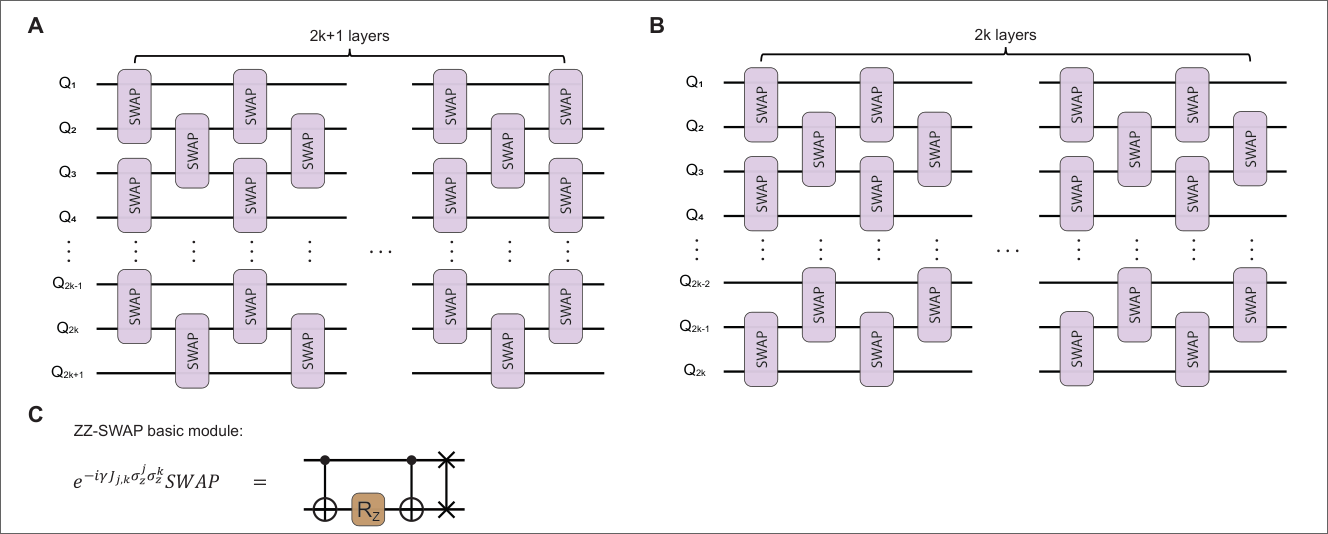
\includegraphics[scale=0.35]{inc/fig_12.png}
    \caption{
    Схема параллельной пузырьковой сортировки, реализующей обратную
    перестановку. A — случай нечётного числа кубитов, B — случай чётного числа
    кубитов. В обоих случаях количество слоёв внешнего цикла составляет $n$,
    что приводит к глубине схемы $O(n)$. C — базовый модуль ZZ-SWAP: это
    квантовая схема глубины 4, представляющая собой операцию SWAP, выполненную
    после базового модуля ZZ.
    }
    \label{fig:fig12}
\end{figure}

Кроме того, поскольку каждый ZZ-член в $K_n$ становится модулем ZZ-SWAP,
требуется дополнительная нагрузка в виде $n(n-1)/2$ операций SWAP и глубины $n$
после внедрения. После выполнения схемы порядок кубитов окажется обратным, и
его можно восстановить, снова запустив схему QAOA.

Система с решётчатой топологией (lattice topology) также известна как двумерная
квадратная решётка (2DSL), в которой кубиты располагаются в виде двумерной
решётки, и разрешены только соседние взаимодействия. Поскольку одномерная
цепочка может быть непосредственно вложена в двумерную решётку (например, вдоль
одной из диагоналей или рядов), глубина внедрённой схемы для гамильтониана типа
$K_n$ не будет превышать глубину в случае LNN. Следовательно, справедливо
следующее следствие.

\textbf{Следствие 1.} Глубина схемы для гамильтониана типа $K_n$, внедрённой в
двумерную квадратную решётку (2DSL), составляет $O(n)$ и не требует
дополнительных кубитов.

Топология полного графа является идеальной топологией: схема гамильтониана типа
$K_n$ может быть внедрена оптимально по глубине $O(n)$ без каких-либо
дополнительных квантовых ресурсов. Для топологии LNN необходима дополнительная
глубина $O(n)$. Поскольку схема внедрения на основе параллельной пузырьковой
сортировки также имеет сложность $O(n)$, она является оптимальной как для LNN,
так и для 2DSL-систем в смысле нотации $\mathcal{O}$. Кроме того, в
работе~\cite{cite_55} предложен более эффективный метод внедрения гамильтониана
типа $K_n$ в систему 2DSL с дополнительной глубиной $O(\sqrt{n})$, что
достигается за счёт удобной двумерной структуры.

\subsection*{Оценка ресурсов для факторизации RSA-2048}

В этом разделе мы обсуждаем необходимые квантовые ресурсы для атаки на реальные
RSA-числа на основе полученных выше результатов. Поскольку внедрение схемы не
требует дополнительных кубитов, количество кубитов, необходимое для
факторизации $m$-битного числа, оценивается как $n = \frac{2m}{\log m}$ (здесь
параметр точности $c = 1$). Глубина внедрённой схемы для гамильтониана типа
$K_n$ составляет $3n$ для полностью связанной системы, $4n$ — для системы с
линейной топологией (LNN) и $3n + \sqrt{n}$ — для двумерной решётки (2DSL),
согласно Donny Cheung и соавт.~\cite{cite_55}. Эти оценки получены без учёта
особенностей компиляции базового модуля ZZ (или ZZ-SWAP) в конкретной
физической реализации. В качестве примера рассмотрим RSA-2048. Число кубитов:
$\frac{2 \cdot 2048}{\log 2048} \approx 372$. Глубина схемы однослойного
алгоритма QAOA составляет приблизительно $3n + 2 = 1118$ в полностью связанной
системе, где 2 дополнительных уровня приходятся на однокубитные операции: один
уровень для $R_z$-вращений и один — для $R_x$-вращений. а для двумерной
квадратной решётки (2DSL) — около $3n + \sqrt{n} + 2 = 1139$. Необходимые
квантовые ресурсы для факторизации RSA-чисел различной длины приведены в
Таблице З.10.

\begin{table}[H]
\centering
\caption{
    Оценка квантовых ресурсов для RSA-чисел. Основные квантовые ресурсы,
    рассматриваемые здесь, — это количество кубитов и глубина квантовой схемы
    однослойного алгоритма QAOA в трёх типичных топологиях: полностью связанной
    системе ($K_n$), двумерной решётке (2DSL) и одномерной цепочке (LNN).
    Полученные результаты не учитывают особенности компиляции базового модуля
    ZZ (или модуля ZZ-SWAP) в конкретной физической реализации.
}
\begin{tabular}{c|c|c|c|c}
\hline
\hline
\textbf{RSA } & \textbf{Кубиты} & \textbf{Kn глубина} & \textbf{2DSL глубина} & \textbf{LNN глубина} \\
\hline
RSA-128  &  37  & 113  & 121  & 150 \\
RSA-256  &  64  & 194  & 204  & 258 \\
RSA-512  & 114  & 344  & 357  & 458 \\
RSA-1024 & 205  & 617  & 633  & 822 \\
RSA-2048 & 372  & 1118 & 1139 & 1490 \\
\hline
\hline
\end{tabular}
\end{table}

Мы также проанализировали масштаб RSA-чисел, а именно предельный размер
(touch-size), которого могут достичь современные квантовые вычислительные
устройства при некоторых идеальных условиях, при которых все заявленные кубиты
считаются относительно идеальными или обладающими высокой достоверностью.
Результаты приведены в соответствии с топологией связности кубитов квантовых
устройств с использованием алгоритма SQIF. Рассматриваемые квантовые процессоры
включают: Sycamore, Eagle, Aspen-M, Zuchongzhi2, Tianmu-1, а также ионные
ловушки, разработанные в Мэриленде и компанией IonQ. Все эти устройства либо
находятся в публичном доступе, либо доступны через облачные квантовые
платформы. Кроме того, мы указываем минимальную необходимую глубину схемы
(``depth-least'') для этих устройств, при которой можно попытаться
факторизовать RSA-числа предельного размера. Эта глубина оценивается по глубине
однослойной схемы QAOA.В частности, если квантовый процессор имеет двумерную
решётчатую топологию, глубина схемы рассчитывается по модели 2DSL. Для
топологий типа ``прочие'' глубина рассчитывается по модели LNN. Подробные
результаты приведены в Таблице З.11.

Из Таблицы З.11 видно, что предельный размер для устройств NISQ уже близок к
реальным RSA-числам. Например, 127-кубитная машина \texttt{ibm-eagle} имеет
предельный размер 581, а минимально необходимая глубина схемы составляет 510.
Это означает, что если все кубиты функционируют стабильно и обеспечивают
достаточную точность после 510 уровней схемы, устройство может быть
использовано для попытки факторизации RSA-581.

Тем не менее, предельный размер — это идеализированная оценка. На практике
алгоритм QAOA обычно требует более чем одного слоя, что увеличивает глубину
схемы. Кроме того, наличие квантового ускорения по-прежнему остаётся
неизвестным, и квантовый взлом RSA пока остаётся далёкой целью.

\begin{table}[ht]
\centering
\caption{
    Предельный размер RSA-чисел для некоторых известных квантовых устройств.
    Результаты приведены на основе топологии связности кубитов и набора базовых
    логических затворов соответствующих квантовых устройств, с использованием
    предложенного нами алгоритма. Последний столбец указывает минимальное
    условие по глубине схемы, которое должно быть выполнено для возможности
    факторизации. Для систем с топологией типа ``прочие'' глубина схемы
    рассчитывается по модели LNN.
    }
\resizebox{\textwidth}{!}{%
\begin{tabular}{|c|c|c|c|c|c|}
\hline
\textbf{Система} & \textbf{Устройство} & \textbf{Кубиты} & \textbf{Топология} & \textbf{Предельный размер} & \textbf{Мин. глубина} \\
\hline
\multirow{4}{*}{Сверхпроводящие кубиты}
& Sycamore      & 53  & 2DSL   & 201 & 170 \\
& Eagle         & 127 & прочие & 581 & 510 \\
& Aspen-M       & 80  & прочие & 334 & 322 \\
& Zuchongzhi2   & 66  & 2DSL   & 264 & 210 \\
& Tianmu-1      & 36  & 2DSL   & 124 & 118 \\
\hline
\multirow{2}{*}{Ионные ловушки}
& Maryland      & 40  & $K_n$  & 142 & 122 \\
& IonQ          & 79  & $K_n$  & 329 & 239 \\
\hline
\end{tabular}
}
\label{tab:device_resources}
\end{table}

\end{document}
